\phantomsection
\chapter{Dependensee}
\markboth{Dependensee}{}
\label{cap5:dependensee}
% [titolo ridotto se non ci dovesse stare] 
\begin{center}
    
\includegraphics[width=.5\columnwidth]{capitoli/figure/logo_dependensee}
\end{center}

In questo capitolo verr\`{a} introdotto \textit{Dependensee}, lo strumento sviluppato per la visualizzazione di insiemi minimali di \acrlong{rfds} mediante l'implementazione della metafora visiva descritta nel paragrafo \ref{section:visual_rep_metaphore}. Tale strumento facilita la visualizzazione delle \acrlong{rfds} minimali e rappresenta diverse loro caratteristiche, facilitando l'utente nell'analisi visiva degli insiemi composti da queste.

\section{Introduzione} %\label{1sec:scopo}
Dependensee \`{e} una web application che mira a rappresentare visivamente grandi insiemi minimali di \acrlong{rfds}, per permettere all'utente che lo utilizza una rapida e semplice analisi visiva di questi insiemi. Ci\`{o} avviene attraverso una metafora intuitiva, descritta in dettaglio nel capitolo \ref{section:visual_rep_metaphore}, la quale fornisce una panoramica generale sull'insieme, esplicitando dettagli e caratteristiche delle \acrlong{rfds} che formano l'insieme. Per quanto concerne lo sviluppo sono state utilizzate diverse tecnologie, le quali verranno esposte pi\'{u} nel dettaglio nel paragrafo \ref{tecnologie}, tra cui \textit{D3.js}. Il tool trasforma i dati testuali in grafici immediati tramite la manipolazione di questa libreria, la quale permette di costruire grafici complessi in formato SVG. Dependensee \`{e} stato sviluppato con l'obiettivo di semplificare e velocizzare l'analisi dei dataset, infatti, presenta un'interfaccia semplice e pulita, che non richiedere particolari conoscenze. Ci\`{i} \`{e} vero anche per il suo funzionamento, di fatti sono poche le azioni da eseguire per analizzare un dataset ed ottenere il grafico relativo, e per l'interpretazione della rappresentazione grafica dei risultati.

\section{Tecnologie utilizzate}\label{tecnologie}
Per lo sviluppo di Dependensee \`{e} stato utilizzato il pattern Model-View-Controller (MVC), in modo tale da separare la logica di presentazione con la logica di business, con le seguenti tecnologie:
\begin{itemize}
    \item TypeScript,
    \item Angular,
    \item Ionic,
    \item D3.js,
    \item Node.js.
\end{itemize}
% -- Pattern MVC
\begin{figure}[ht]
    \centering
    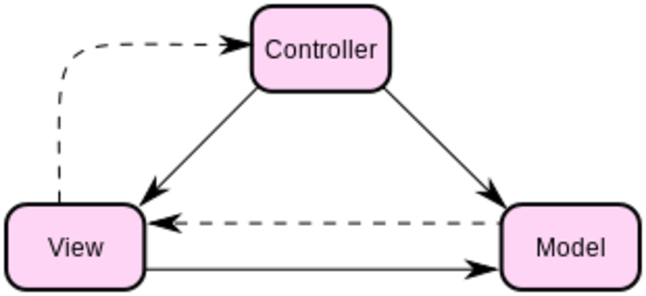
\includegraphics[width=.5\columnwidth]{capitoli/figure/mvc}
    \caption{Pattern Model-View-Controller (MVC).}
    \label{fig:pattern_mvc}
\end{figure}
% -- End Pattern MVC
Il pattern MVC \`{e} un pattern architetturale in grado di separare la logica di presentazione con la logica di business. Esso \`{e} composto da tre componenti diversi tra loro: Model, View e Controller.
Il Model fornisce i metodi per accedere ai dati utili all'applicazione, la View visualizza i dati contenuti nel Model e si occupa dell'interazione con gli utenti, mentre il Controller riceve i comandi dall'utente attraverso la View e li attua modificando lo stato degli altri due componenti. Il pattern appena descritto lo troviamo anche in Angular, evoluzione di AngularJS, il quale \`{e} un framework open source per lo sviluppo di applicazioni web. Le applicazioni sviluppate mediante Angular sono supportate su tutti i principali web browser, da computer a mobile, e vengono eseguite internamente nel browser dopo essere state scaricate dal server. Tale framework \`{e} sviluppato da Google ed il linguaggio di programmazione utilizzato \`{e} TypeScript, lo troviamo alla base di Ionic e costituisce il lato back-end dell'applicazione. TypeScript \`{e} un linguaggio di programmazione open source sviluppato dalla Microsoft, nato dal crescente bisogno di un linguaggio front-end per lo sviluppo di applicazioni JavaScript su larga scala. Si tratta, infatti, di un superset di JavaScript che basa le sue caratteristiche su ECMAScript 6. Esso estende la sintassi di JavaScript, in questo modo qualunque programma scritto in JavaScript \`{e} anche in grado di essere eseguito con TypeScript senza alcuna modifica. Inoltre, \`{e} stato progettato principalmente per lo sviluppo di applicazioni e viene successivamente ricompilato in JavaScript per poter essere interpretato in qualsiasi web browser e su qualsiasi sistema operativo. Ionic \`{e} un Software Development Kit (SDK) open source completo per lo sviluppo di app ibride e costituisce principalmente il lato front-end dell'applicazione. Esso fornisce strumenti e servizi per lo sviluppo di applicazioni desktop, mobile e Progressive Web Apps, basate sulle pratiche e tecnologie moderne di sviluppo web, utilizzando tecnologie come CSS, HTML5 e SASS. In particolare, possono essere sviluppate applicazioni mobile con le suddette tecnologie web ed \`{e} possibile, successivamente, distribuirle tramite Cordova o Capacitor sui vari App Store nativi. D3.js \`{e} una libreria sviluppata in JavaScript per creare visualizzazioni dinamiche ed interattive partendo da dati organizzati, visibili attraverso un comune browser. Per fare ci\`{o} si serve largamente degli standard web: SVG, HTML5, CSS. Diversamente da molte altre librerie, essa permette un ottimo controllo e resa visiva sul risultato finale. D3.js, incorporata in una pagina web HTML, utilizza funzioni JavaScript prefatte per selezionare elementi del DOM, creare elementi SVG, aggiungergli uno stile grafico, oppure transizioni, effetti di movimento e/o tooltip. In questo modo grandi collezioni di dati possono essere facilmente convertiti in oggetti SVG usando semplici funzioni della libreria e generare cos\`{i} ricche rappresentazioni grafiche di numeri, testi, mappe e diagrammi. I dati utilizzati possono essere in diversi formati, i pi\`{u} comuni sono JSON e CSV, ma, se necessario, si possono scrivere funzioni per leggere dati in altri formati. Il tutto viene eseguito su Node.js, una runtime di JavaScript open source multipiattaforma orientato agli oggetti per l'esecuzione di codice JavaScript. Node.js permette di implementare il cosiddetto paradigma \textit{"JavaScript everywhere"}, unificando lo sviluppo su un unico linguaggio di programmazione, ovvero JavaScript, sia per il lato client che per il lato server. Esso ha un'architettura orientata agli eventi che rende possibile l'I/O asincrono e migliora il throughput e la scalabilit\`{a} nelle applicazioni web con molte operazioni di input/output.

\section{Implementazione}
L'applicazione Dependensee \`{e} stata implementata sulla base del pattern MVC, descritto in precedenza, e si compone principalmente di:
\begin{itemize}
    \item Homepage,
    \item Visualize Page,
    \item Analyzer Service.
\end{itemize}
La prima componente, ovvero l'homepage, attualmente rimanda direttamente alla Visualize Page, di cui parleremo a breve. Prima \`{e} necessario introdurre l'implementazione effettiva di una \acrlong{rfd} all'interno di Dependensee.\par
Per l'implementazione delle \acrshort{rfds} \`{e} stata creata una classe, \textit{RelaxedFunctionalDependence}, la quale definisce una \acrshort{rfd} come un oggetto con due attributi:
\begin{lstlisting}[language=java, numbers=left, xleftmargin=3em, captionpos=b, caption={Implementazione delle \acrshort{rfds} in Dependensee.}, frame=lines]
export class RelaxedFunctionalDependence {
    private lhs: Array<[string, number]>;
    private rhs: [string, number];
    ...
}
\end{lstlisting}
\begin{itemize}
    \item \texttt{lhs} \`{e} un array di tuple del tipo \texttt{[string,number]}, il quale contiene gli attributi del lato sinistro della \acrshort{rfd} con le relative thresholds,
    \item \texttt{rhs} \`{e} una tupla del tipo \texttt{[string,number]} che contiente l'attributo del lato destro della \acrshort{rfd} con la threshold relativa.
\end{itemize}
Visualize Page \`{e} composta da due elementi: \texttt{visualize.page.html} che rappresenta la View per l'interazione con l'applicazione, \texttt{visualize.page.ts} che rappresenta il Model. Nella View \`{e} presente un'interfaccia semplice e pulita, dove \`{e} richiesto il dataset da analizzare in formato \texttt{.txt} e la threshold massima. Inoltre, sempre nella View, \`{e} presente un area di log a scomparsa dove \`{e} possibile leggere i messaggi di log ed un'area alla fine della pagina dove appare il grafico risultante dall'analisi. Il Model, ovvero \texttt{visualize.page.ts}, si interpone tra la View ed il Controller, utilizza i metodi dell'Analyzer Service per analizzare i dati e crearne poi un grafico da inserire all'interno della View in modo dinamico. La creazione del grafico avviene mediante due metodi definiti come \texttt{drawMatrix} e \texttt{plotCell}.
Il metodo \texttt{drawMatrix} \`{e} il metodo principale, questo ha il compito di creare l'oggetto SVG nella View, il quale conterr\`{a} il grafico finale. Il metodo si occupa di creare l'oggetto SVG all'interno della View, creare tutte le label da disegnare nell'oggetto SVG e, inoltre, creare le singole celle non facenti parte della diagonale attraverso la chiamata al metodo \texttt{plotCell}. Il metodo \texttt{plotCell} viene chiamato solamente da \texttt{drawMatrix} per ogni sotto-matrice del grafico non facenti parte della diagonale. Il metodo per prima cosa disegna gli assi delle ordinate e delle ascisse, relativi alla threshold ed alla cardinalit\`{a}. Definisce poi i colori di riempimento e del bordo del quadrato da posizionare all'interno della sotto-matrice. Fatto ci\`{o}, va a disegnare effettivamente i dati gi\`{a} analizzati tramite l'Analyzer Service, assegnando i colori di riempimento e del bordo in base ai valori di threshold e cardinalit\`{a}.\par
\begin{lstlisting}[numbers=left, xleftmargin=3em, captionpos=b, caption={Pseudocodice del metodo per il parsing dei dataset.}, label=analyzeFile_pseudo, frame=lines, breaklines=true, morekeywords={if, then, else, end, to, do, for}]
if file.formato != .txt then
    errore, formato non valido
else if numeroRighe < 1 then
    errore, file vuoto
else
    istanzia rfdSet
    for i = 0 to numeroRighe do
        if riga[i] contiene '@' then
            esegui lo split della riga[i] con '->'
            esegui lo split della riga[i][1] con ','
            istanzia lhsA come riga[i][1] derivata dallo split con '@'
            istanzia rhsA come riga[i][2] derivata dallo split con '@'
            istanzia rfd
            rfd.lhs = lhsA
            rfd.rhs = rhsA
            rfdSet = rfdSet + rfd
        end if
    end for
end if
\end{lstlisting}
L'Analyzer Service rappresenta il Controller ed al suo interno vi sono due metodi principali invocati dal Model.
Il primo metodo si occupa del parsing del dataset inserito in input dall'utente e lo pseudoalgoritmo relativo \`{e} esposto nel Listing 5.2. La prima operazione da effettuare \`{e} il controllo del formato del dataset e ci\`{o} avviene nelle righe 1-2. Questa operazione risulta cruciale in quanto Dependensee opera su dataset che hanno struttura e formato noti. La seconda operazione, anch'essa importante, \`{e} il controllo del contenuto del file, righe 3-4. Se il numero delle righe del file dovesse risultare minore di $1$ allora vorr\`{a} dire che il dataset sar\`{a} vuoto. La terza operazione ed ultima operazione, righe 5-18, \`{e} il parsing effettivo dei dataset. Si istanzia rfdSet, riga 6, il quale \`{e} un insieme che conterr\`{a} le \acrshort{rfds} contenute nel dataset. La struttura di una \acrshort{rfd} contenuta nel dataset \`{e} \texttt{A$_1$@T$_1$,A$_2$@T$_2$,...,A$_n$@T$_n$->A@T}. Detto ci\`{o}, per ogni riga del dataset, se queste contengono il simbolo chiocciola (\texttt{@}), si effettuano diverse operazioni:
\begin{itemize}
    \item la prima operazione \`{e} lo split, ovvero la divisione, della riga utilizzando come riferimento la sequenza di caratteri '\texttt{->}' (riga 9),
    \item la prima met\`{a} della riga viene divisa prima utilizzando come riferimento il carattere '\texttt{,}', creando cos\`{i} una lista di sottostringhe del tipo \texttt{A@T}, poi viene ulteriormente divisa utilizzando come riferimento il carattere '\texttt{@}', creando cos\`{i} una lista di sottostringhe corrispondenti agli attributi con le relative thresholds associate (righe 10-11),
    \item la seconda met\`{a} della riga viene ulteriormente divisa esattamente come la prima met\`{a}, ottenendo cos\`{i} una lista di sottostringhe corrispondenti agli attributi con le relative thresholds associate (riga 12),
    \item viene istanziato un oggetto con due attributi, lhs e rhs, che rappresenta una \acrshort{rfd}. Ai suoi due attributi lhs e rhs vengono assegnate le stringhe derivate dallo split ed assegnate alle variabili \texttt{lhsA} e \texttt{rhsA} (righe 13-15),
    \item infine, viene aggiunta la \acrshort{rfd} all'interno dell'insieme \texttt{rfdSet} (riga 16).
\end{itemize}
L'implementazione di tale algoritmo \`{e} risultata efficace per il parsing dei dati che avviene senza alcun tipo di errore. Il secondo metodo si occupa della propagazione dei dati ottenuti dal parsing dei dataset. Questo metodo, il cui pseudocodice \`{e} esposto nel Listing 5.3, viene invocato per la costruzione di ogni sotto-matrice della rappresentazione visiva, prendendo in input l'insieme delle \acrshort{rfds} (\texttt{rfdSet}), l'attributo del lato sinistro e del lato destro (\texttt{lhsAttribute}, \texttt{rhsAttribute}) relativi alla sotto-matrice che si sta costruendo, la threshold massima data in input dall'utente (\texttt{maxThreshold}) e la cardinalit\`{a} massima (\texttt{maxCardinality}). La propagazione avviene nel seguente modo:
\begin{itemize}
    \item prima si istanza una matrice vuota $\imath \times \jmath$, dove $\imath$ \`{e} uguale a \texttt{maxThreshold} e $\jmath$ \`{e} uguale a \texttt{maxCardinality} (riga 1),
    \item per ogni elemento della matrice si istanzia prima una \acrshort{rfd} temporanea vuota per effettuare gli scambi e per ogni \acrshort{rfd} contenuta nell'insieme \texttt{rfdSet}, se queste contengono gli attributi indicati su ambo i lati (\texttt{lhsAttribute}, \texttt{rhsAttribut}), vengono comparate con la \acrshort{rfd} temporanea: se l'attributo sul lato sinistro \`{e} maggiore di quello della \acrshort{rfd} temporanea, minore della threshold massima e la cardinalit\`{a} \`{e} uguale a $\jmath$, allora avviene lo scambio. In questo modo, la \acrshort{rfd} temporanea contiene la dipendenza minima (righe 4-11),
    \item qualora non dovessero esserci \acrshort{rfd} minimali che rispettano quelle condizioni (dettate da $\imath$ e $\jmath$ che ciclano) allora nella matrice ci sar\`{a}: la propagazione della \acrshort{rfd} sottostante se si sta analizzando la prima colonna, la propagazione della \acrshort{rfd} precedente nel caso in cui si sta analizzando la prima riga, altrimenti la propagazione della \acrshort{rfd} che risulta essere minimale tra quella precedente e quella sottostante (righe 12-19),
    \item infine, il metodo restituisce la matrice in output (riga 22).
\end{itemize}
\begin{lstlisting}[numbers=left, xleftmargin=3em, captionpos=b, caption={Pseudocodice del metodo per la propagazione dei dati.}, label=retrieveData_pseudo, frame=lines, breaklines=true, morekeywords={if, then, else, end, to, do, for, of}]
istanzia la matrice vuota rfdMatrix
for i = 0 to maxThreshold do
    for j = 1 to maxCardinality do
        istanzia una rfd temporanea in rfdTemp
        for rfd of rfdSet do
            if rfd contiene lhsAttribute e rhsAttribute then
                if rfdTemp < rfd.lhsAttribute < maxThreshold e rfd.cardinality = j then
                    rfdTemp = rfd
                end if
            end if
        end for
        if non esistono rfd then
            if stai analizzando la prima colonna then
                propaga il dato sottostante in rfdTemp
            else if stai analizzando la prima riga then
                propaga il dato precedente in rfdTemp
            else propaga il dato minimale tra il precedente ed il sottostante in rfdTemp
        end if
        rfdMatrix[i][j] = rfdTemp
    end for
end for
restistuisci rfdMatrix
\end{lstlisting}\par
Riassumendo: il primo metodo, si occupa di analizzare il dataset ricevuto in input e restituisce in output un oggetto \texttt{rfdSet}, il quale \`{e} un array del tipo \textit{RelaxedFunctionalDependence} che contiene tutte le dipendenze riscontrare nel dataset, ed un oggetto \texttt{attributes}, il quale \`{e} un array di stringhe che contiene tutti gli attributi individuati nel dataset. Il suo funzionamento si basa sulla lettura del dataset, riga per riga, tramite un \texttt{FileReader} e, per ogni riga, si effettuano operazioni di divisione della stringa per individuare gli attributi su ambo i lati con le thresholds relative. Il secondo metodo, dati in input il set di \acrshort{rfds}, gli attributi del lato sinistro e del lato destro, la threshold massima e la cardinalit\`{a} massima, individua le \acrshort{rfds} valide e le restituisce come un oggetto JSON. Questo metodo viene richiamato per ogni sotto-matrice del grafico risultante in fase di creazione, ovvero per individuare i dati relativi ad ogni attributo visto sul lato sinistro per un fissato attributo sul lato destro. Per testare la validit\`{a} di una \acrshort{rfd}, il metodo verifica, in due cicli annidati che corrispondono alla threshold massima ed alla cardinalit\`{a} massima, prima che questa contenga gli attributi indicati in input per il lato sinitro e per il lato destro, poi verifica le thresholds e la cardinalit\`{a}. L'ultima fase di verifica consiste nella propagazione dei dati. La propagazione dei dati avviene quando non esiste una \acrshort{rfd} nel dataset. IL primo caso della propagazione si presenta quando si sta analizzando la prima colonna della matrice e, in questo caso, viene propagata la \acrshort{rfd} sottostante. Il secondo caso della propagazione si presenta quando si sta analizzando la prima riga della matrice e, in questo caso, viene propagata la \acrshort{rfd} precedente. Il terzo ed ultimo caso della propagazione avviene quando si analizza la parte centrale della matrice, qui la propagazione avviene della \acrshort{rfd} minimale tra quella precedente e quella sottostante.

\section{Funzionamento}
Dependensee mira alla semplicit\`{a} ed all'efficacia, ragion per cui presenta un'interfaccia pulita e molto semplice da utilizzare. Il deploy dell'applicazione pu\`{o} essere effettuato sia su server che in locale. Per effettuare il deploy in locale \`{e} necessario, come prerequisiti, avere Node.js, npm ed Ionic 4 sulla propria macchina. Successivamente, basta aprire la directory tramite bash e digitare il comando \texttt{ionic serve}, cos\`{i} da avviare un server in locale su tutte le interfacce di rete. Fatto ci\`{o}, baster\`{a} dirigersi all'indirizzo corrispondente al server avviato, in genere \texttt{http://localhost:8100}, per iniziare ad utilizzare Dependensee. Una volta aperto l'indirizzo nel browser, si presenter\`{a} un'interfaccia semplice ed immediata, come mostrato in Figura \ref{fig:dependensee_main_screen}, composta da:
\begin{itemize}
    \item un input per selezione il dataset da analizzare in formato \texttt{.txt},
    \item un input per indicare la threshold massima,
    \item un bottone per avviare l'analisi e generare il grafico relativo al dataset,
    \item una finestra nascosta di default che \`{e} possibile mostrare per leggere i messaggi di log generati da Dependensee.
\end{itemize}
% -- Main Screen
\begin{figure}[ht]
    \centering
    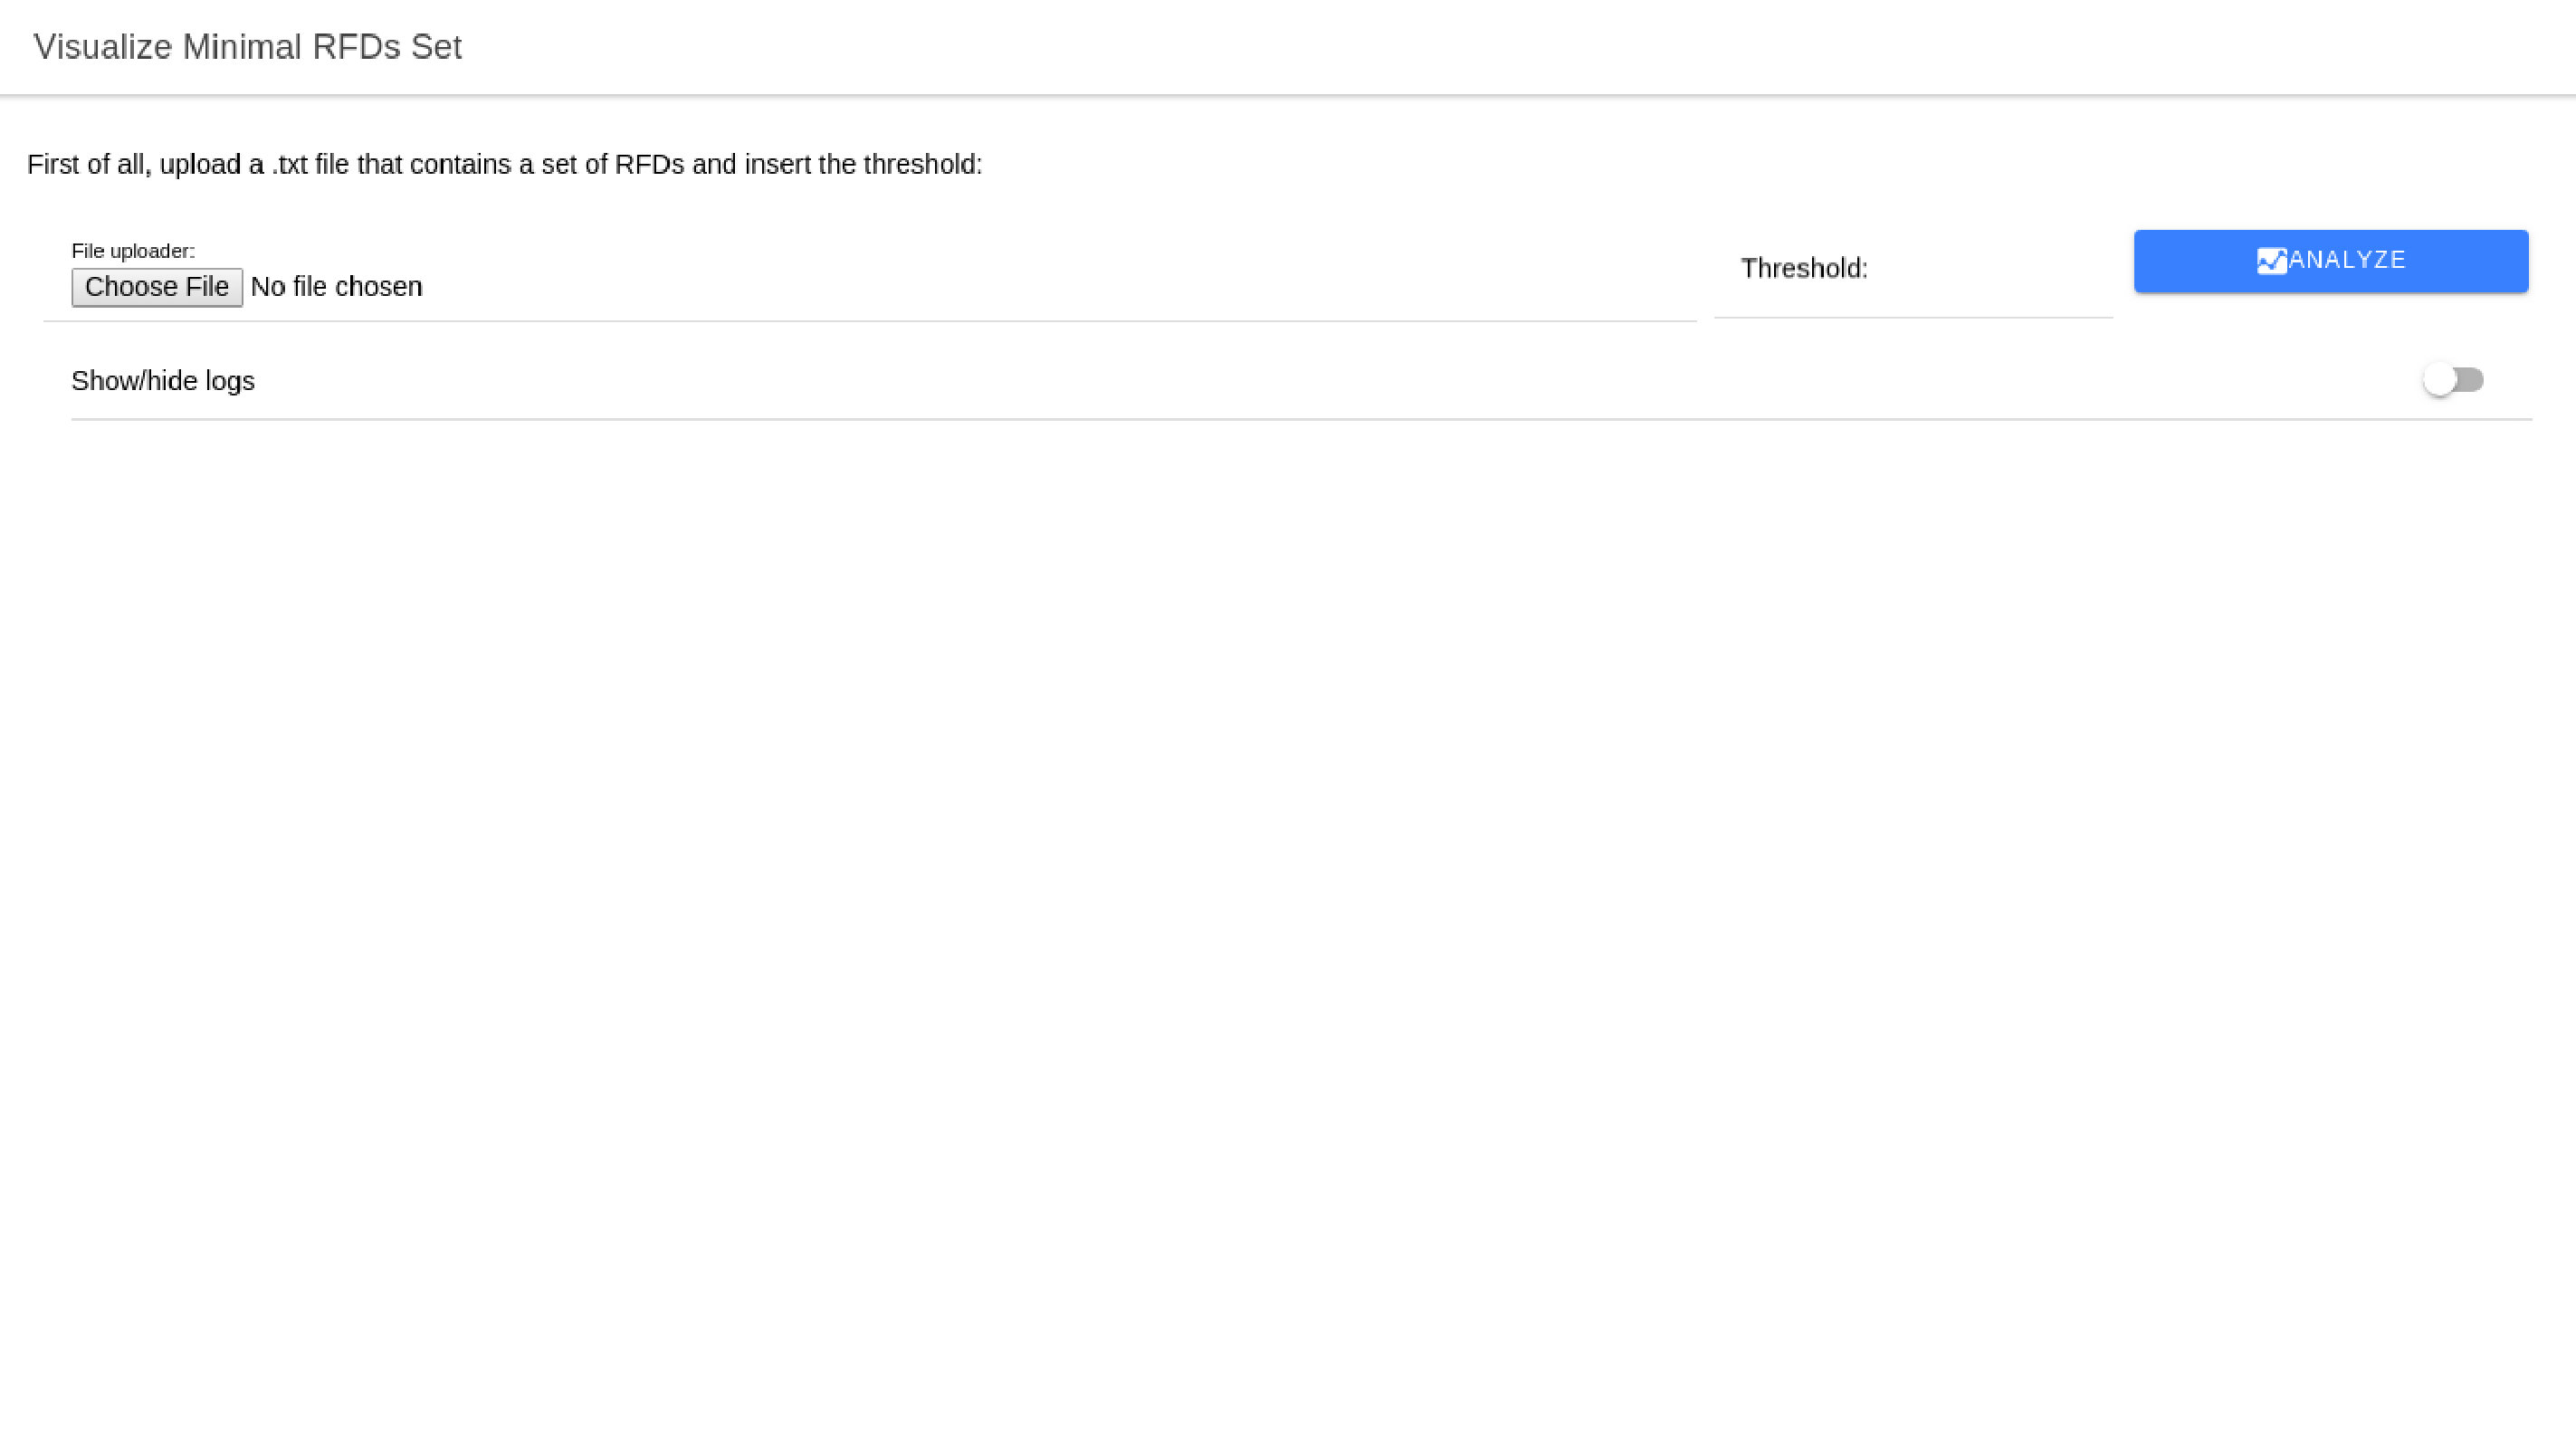
\includegraphics[width=\linewidth]{capitoli/figure/dependensee_main_screen}
    \caption{Interfaccia di Dependensee.}
    \label{fig:dependensee_main_screen}
\end{figure}
% -- End Main Screen
Quindi, bisogna selezionare il dataset da analizzare in formato .txt, con la seguente struttura:
\begin{verbatim}
    B@4.0->F@4.0
    D@4.0->F@4.0
    C@4.0->F@4.0
    E@4.0->F@4.0
    G@4.0->F@4.0
    A@4.0->F@4.0
    A@2.0,B@0.0,C@0.0,D@4.0,E@2.0,F@2.0->G@2.0
    A@0.0,B@0.0,C@0.0,D@4.0,E@2.0,F@2.0->G@0.0
\end{verbatim}
dove le stringhe che precedono il simbolo \texttt{@} indicano gli attributi, i valori che vengono scritti dopo il simbolo \texttt{@} indicano le threshold relative agli attrubuti ed i simboli \texttt{->} dividono il lato sinistro della \acrshort{rfd} dal lato destro. Successivamente, bisogna inserire il valore massimo delle threshold e cliccare sul bottone per avviare l'analisi. Se i due campi di input non sono stati violati, allora Dependensee proceder\`{a} con l'analisi e visualizzer\`{a} un grafico relativo al dataset inserito, come mostrato in Figura \ref{fig:dependensee_dataset_analyzed}, altrimenti mostrer\`{a} un messaggio d'errore relativo al campo di input da modificare.
% -- Dataset Analyzed
\begin{figure}[ht]
    \centering
    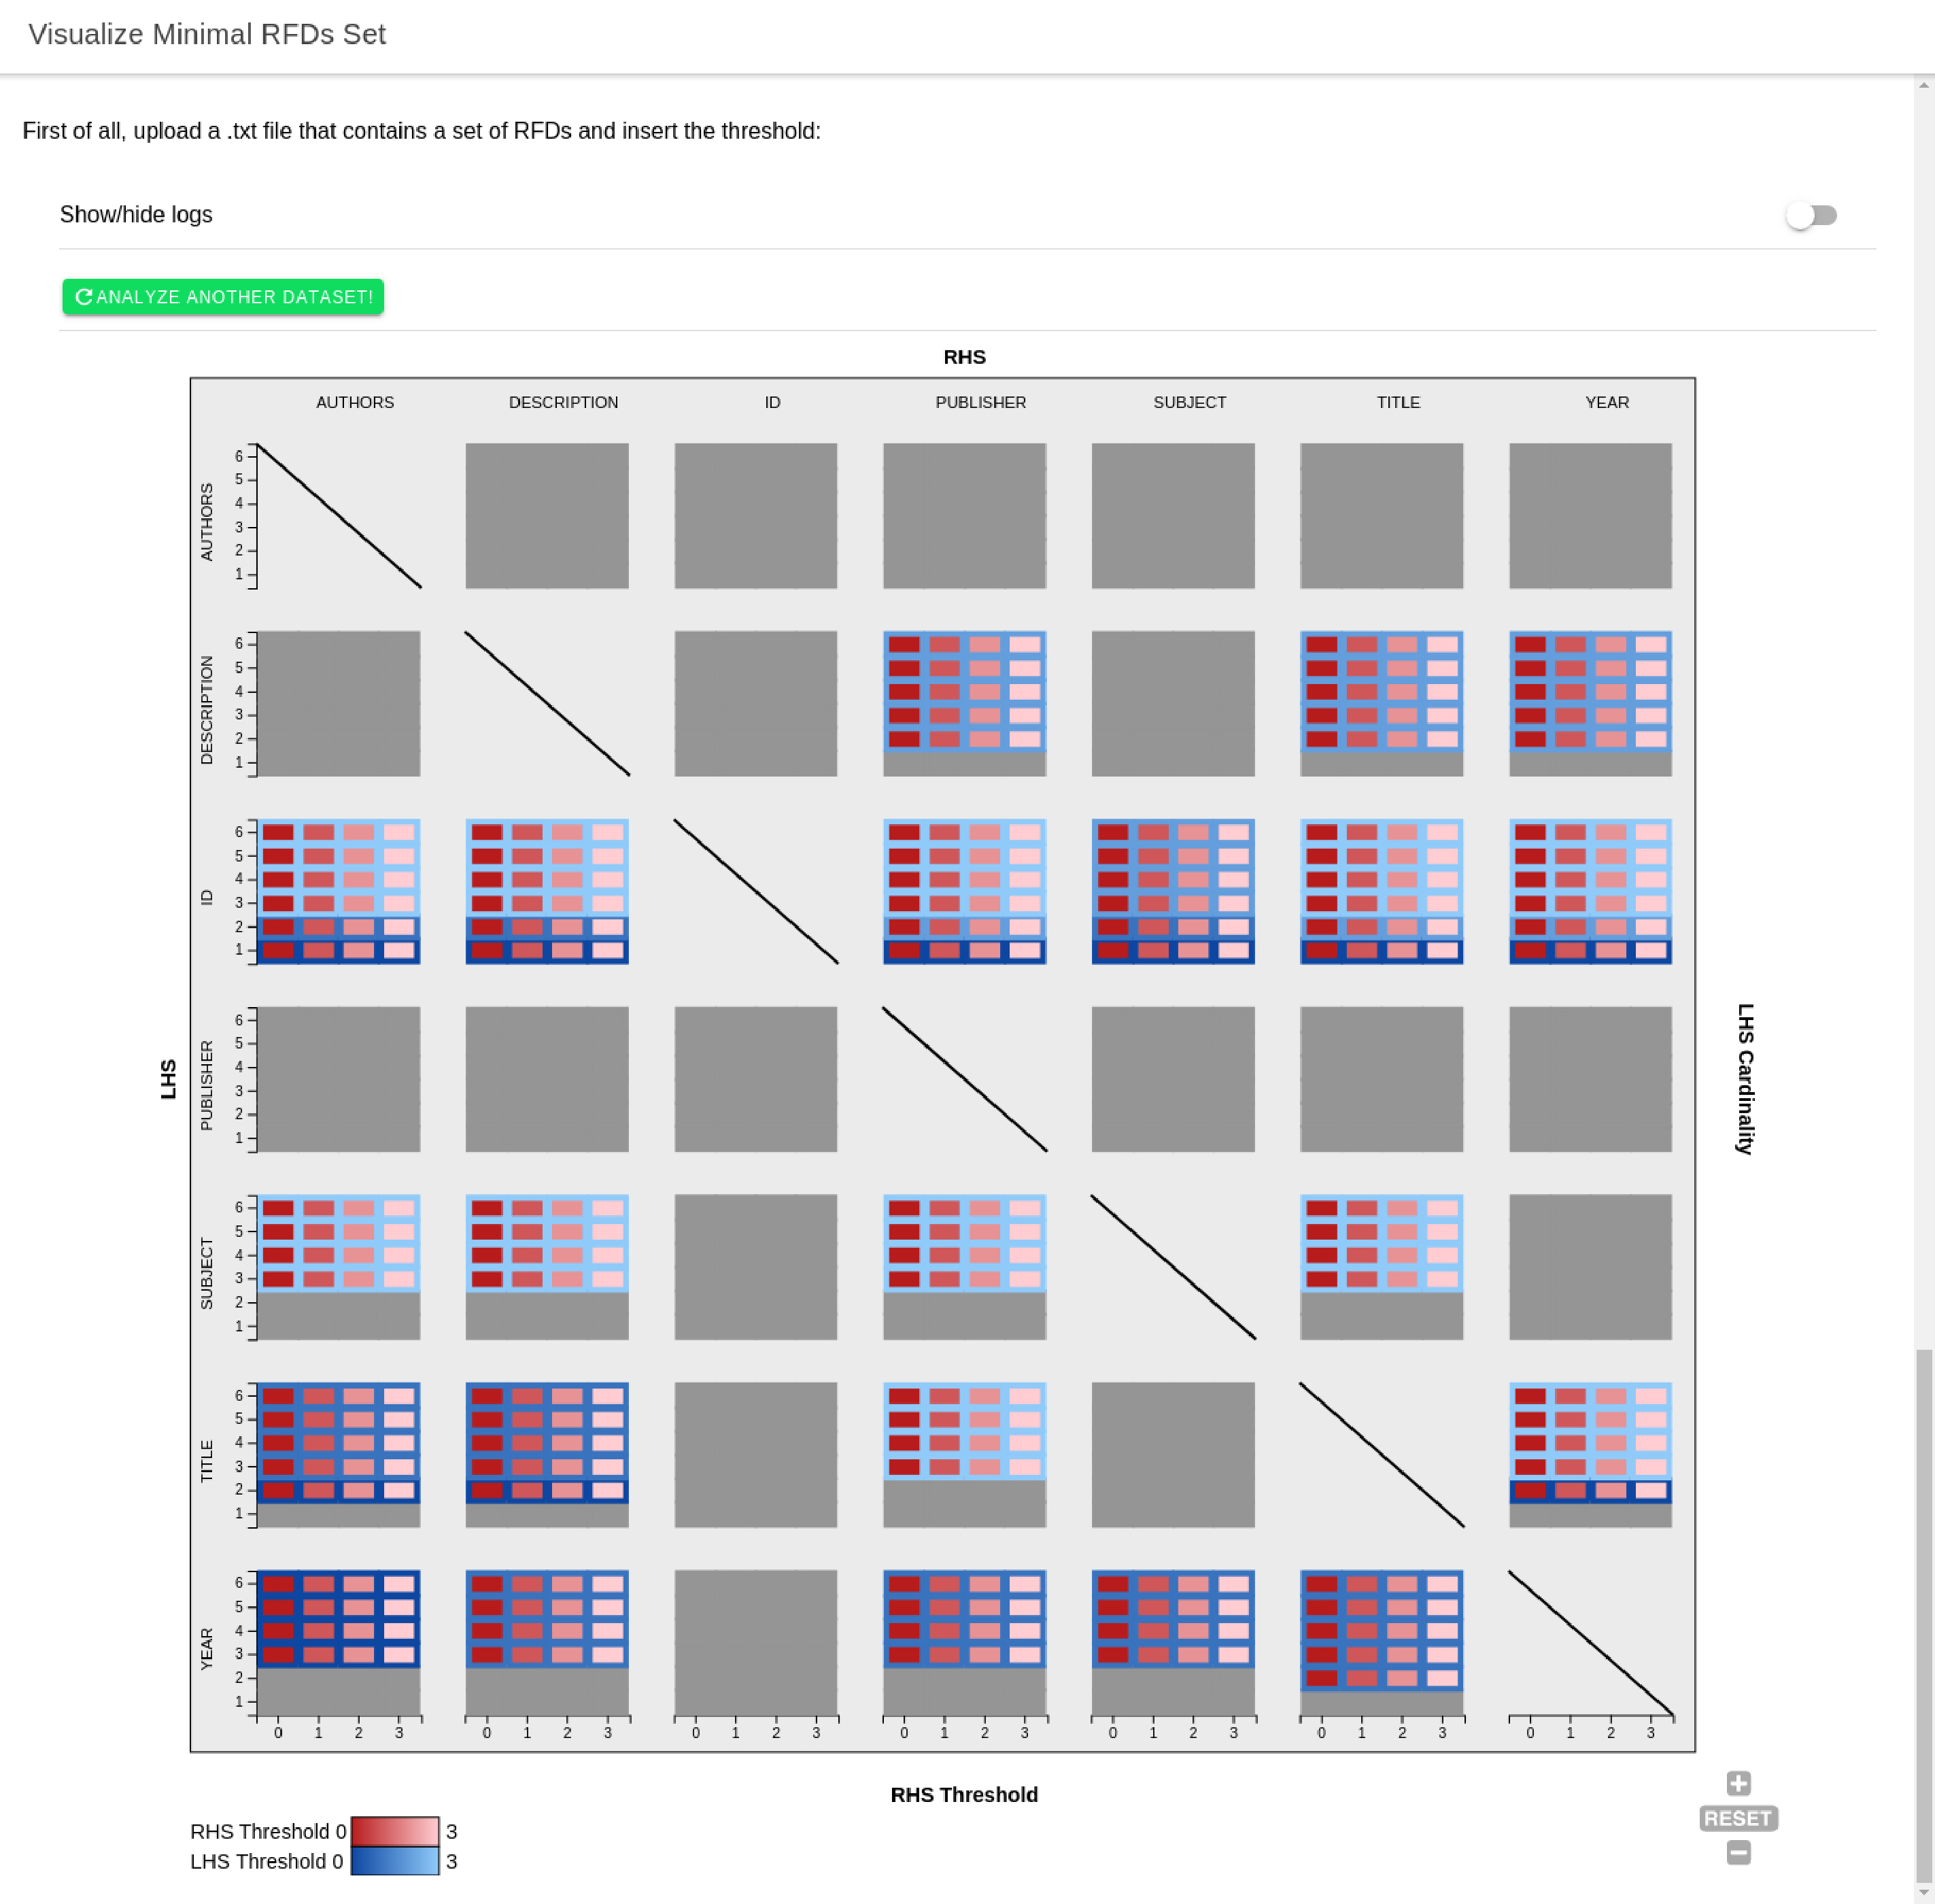
\includegraphics[width=\linewidth]{capitoli/figure/dependensee_analyzed_screen}
    \caption{Grafico generato da Dependensee relativo al dataset inserito in input.}
    \label{fig:dependensee_dataset_analyzed}
\end{figure}
% -- End Dataset Analyzed
Una volta ottenuta la rappresentazione grafica del dataset sar\`{a} possibile effettuare operazioni di zoom-in/out per visualizzarlo meglio e per concentrarsi in singole porzioni di esso, oppure sar\`{a} possibile analizzare un altro dataset cliccando sul bottone in alto.

\section{Interpretazione dei risultati}
Una volta analizzato un dato dataset, il tool proceder\`{a} alla creazione di un grafico colorato con le \acrlong{rfds} contenute nel dataset. Il grafico consiste in una matrice $n\times n$, dove $n$ \`{e} il numero di attributi presenti nel dataset. Gli attributi presenti sulle righe fanno riferimento alle \acrshort{rfds} in cui appare l'attributo in questione sul lato sinistro, mentre gli attributi presenti sulle colonne fanno riferimento alle \acrshort{rfds} in cui appare l'attributo in questione sul lato destro. La matrice \`{e} a sua volta composta da delle sotto-matrici, in cui gli elementi vengono rappresentati seguendo due metriche: cardinalit\`{a} del lato sinistro e threshold dell'attributo sul lato destro. Se ogni sotto-matrice viene vista come un piano cartesiano in due dimensioni, le ascisse rappresentano le thresholds del lato destro, mentre le ordinate rappresentano le cardinalit\`{a} del lato sinistro. I colori utilizzati per raffigurare gli elementi rappresentano la threshold dell'attributo sul lato sinistro e la threshold dell'attributo sul lato destro, rispettivamente il bordo ed il riempimento. Colori pi\`{u} intensi indicano thresholds pi\`{u} vicine o uguali a zero, mentre colori meno intensi indicano threshold pi\`{u} vicine o uguali al valore indicato in input. Ad esempio, se guardiamo il grafico della Figura \ref{fig:dependensee_dataset_analyzed} e consideriamo l'ultima riga e la prima colonna, questa sotto-matrice corrisponde alle \acrshort{rfds} aventi l'attributo \texttt{YEAR} sul lato sinistro e l'attributo \texttt{AUTHORS} sul lato destro. Guardandola possiamo notare l'esistenza di \acrshort{rfds} con cardinalit\`{a} maggiore uguale a $3$, con thresholds sull'attributo \texttt{AUTHORS} comprese tra $0$ e $3$ (inclusi) e thresholds sull'attributo \texttt{YEAR} uguali a $0$. Il colore grigio indica che non esistono \acrshort{rfds} con l'attributo \texttt{YEAR} sul lato sinistro, con l'attributo \texttt{AUTHORS} sul lato destro, con cardinalit\`{a} uguale a $0$ o $1$ e thresholds dell'attributo \texttt{AUTHORS} comprese tra $0$ e $3$.

\section{Valutazione sperimentale}
Attraverso l'implementazione della metafora di visualizzazione esposta nel capitolo \ref{section:visual_rep_metaphore} all'interno di Dependensee, si \`{e} riusciti a rappresentare in modo immediato ed efficace un dataset di \acrlong{rfds}. In questo modo \`{e} stato possibile effettuare un'analisi visiva quasi istantanea, grazie alle diverse caratteristiche messe in luce dalla rappresentazione grafica fornita dallo strumento. Infatti, questa rappresentazione raffigura le dipendenze minimali esistenti tra tutti gli attributi contenute nel dataset, mettendo in risalto la cardinalit\`{a} del lato sinistro e le thresholds associate sia per il lato sinistro che per il lato destro.\par
% -- TAB DATASET --
\begin{table}[ht]
\centering
\begin{tabular}{|lrr|} 
\hline
\multicolumn{3}{|c|}{\textbf{Statistiche }}                                                         \\
\multicolumn{1}{|c}{\textbf{Dataset}} & \multicolumn{1}{c}{\textbf{\#Attributi}} & \textbf{\#RFDs}  \\ 
\hline
Echocardiogram                             & 13                                       & 2396                \\
Restaurant                             & 6                                       & 1961                \\
Citiseer\_2000                        & 7                                       & 107                \\
expIDEAS                             & 3                                       & 12                \\
Foodstamp                             & 5                                       & 9                \\
Car\_Data                             & 7                                       & 8                \\
\hline
\end{tabular}
\caption{Statistiche dei dataset analizzati con Dependensee.}
\label{table:datasets_analyzed_stats}
\end{table}
% -- END TAB DATASET --
La valutazione \`{e} avvenuta attraverso l'analisi dei dataset elencati nella Tabella \ref{table:datasets_analyzed_stats}.
\begin{figure}[ht]
    \centering
    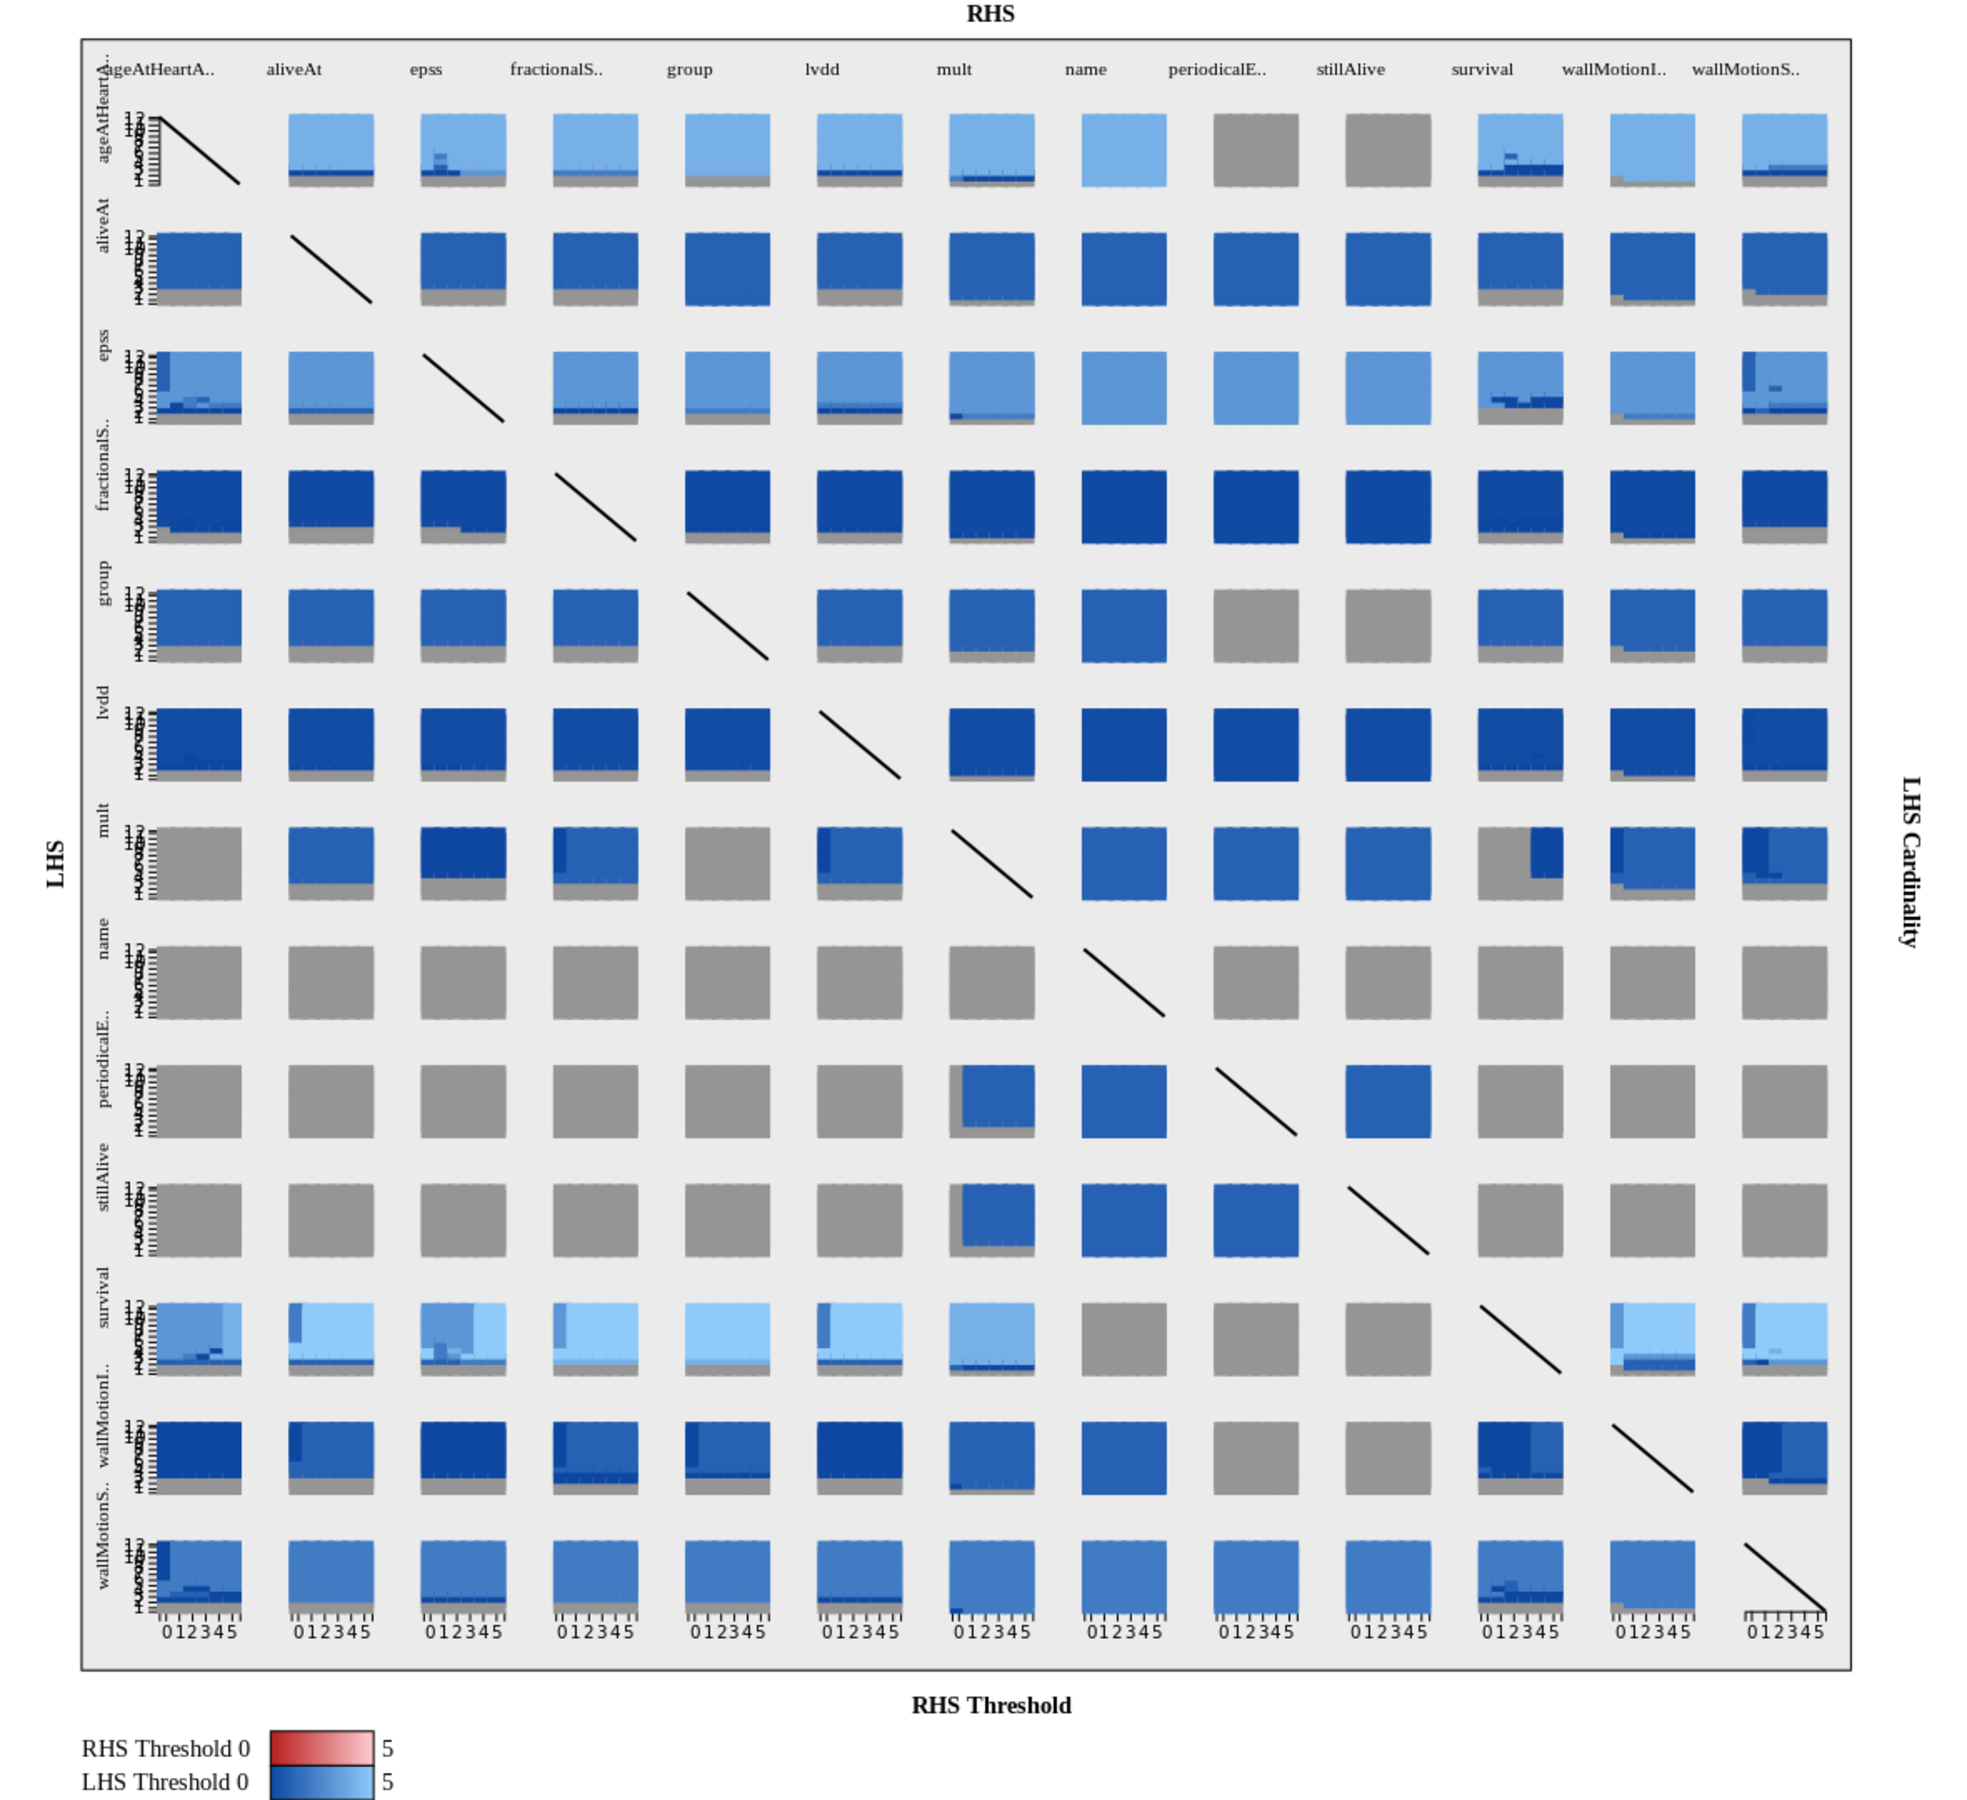
\includegraphics[width=\linewidth]{capitoli/figure/echocardiogram}
    \caption{Rappresentazione ottenuta in output da Dependensee del dataset Echocardiogram.}
    \label{fig:echocardiogram_result}
\end{figure}
La Figura \ref{fig:echocardiogram_result} mostra la rappresentanza grafica ottenuta analizzando il dataset \textit{Echocardiogram} con Dependensee. Da un primo sguardo si pu\`{o} notare come questa faciliti effettivamente l'analisi visiva per l'utente. Analizzando il dataset attraverso tale rappresentazione possiamo notare, mediante la diagonale nulla, come le \acrlong{rfds} banali non vengano rappresentate. In questo caso, data la grande mole di attributi, il grafico risultante enfatizza la threshold del lato sinistra piuttosto che quella del lato destro, essendo quest'ultima fissata. Inoltre, le label di alcuni attributi vengono troncate in quanto troppo lunghe, per evitare che queste si sovrappongano ad altre label. Il dataset \`{e} stato analizzato con una threshold massima data in input pari a $5$. Dalla rappresentazione possiamo notare che non esistono \acrlong{rfds} minimali con l'attributo \texttt{name} sul lato sinistro con threshold tra $0$ e $5$, in quanto tutta la riga \`{e} di color grigio. Se osserviamo, invece, la prima riga e la seconda colonna, possiamo notare l'esistenza di \acrlong{rfds} minimali di cardinalit\`{a} $3$ con threshold minima e le \acrlong{rfds} minimali con cardinalit\`{a} maggiore sono tutte con threshold massima. Se consideriamo la riga con l'attributo \texttt{ageAtHearthAttack} sul lato sinistro e la colonna con l'attributo \texttt{name} sul lato destro, ovvero prima riga ed ottava colonna, possiamo notare che tutte le \acrlong{rfds} minimali sono con threshold massima pari a $5$, difatti tutta la matrice presenta il colore pi\`{u} chiaro. Da un'analisi generale, invece, si pu\`{o} notare che la gran parte delle \acrlong{rfds} minimali sono con threshold minima pari a $0$, molte con threshold medio tra $0$ e $5$, poche con threshold pari al valore massimo $5$.\par
\begin{figure}[ht]
    \centering
    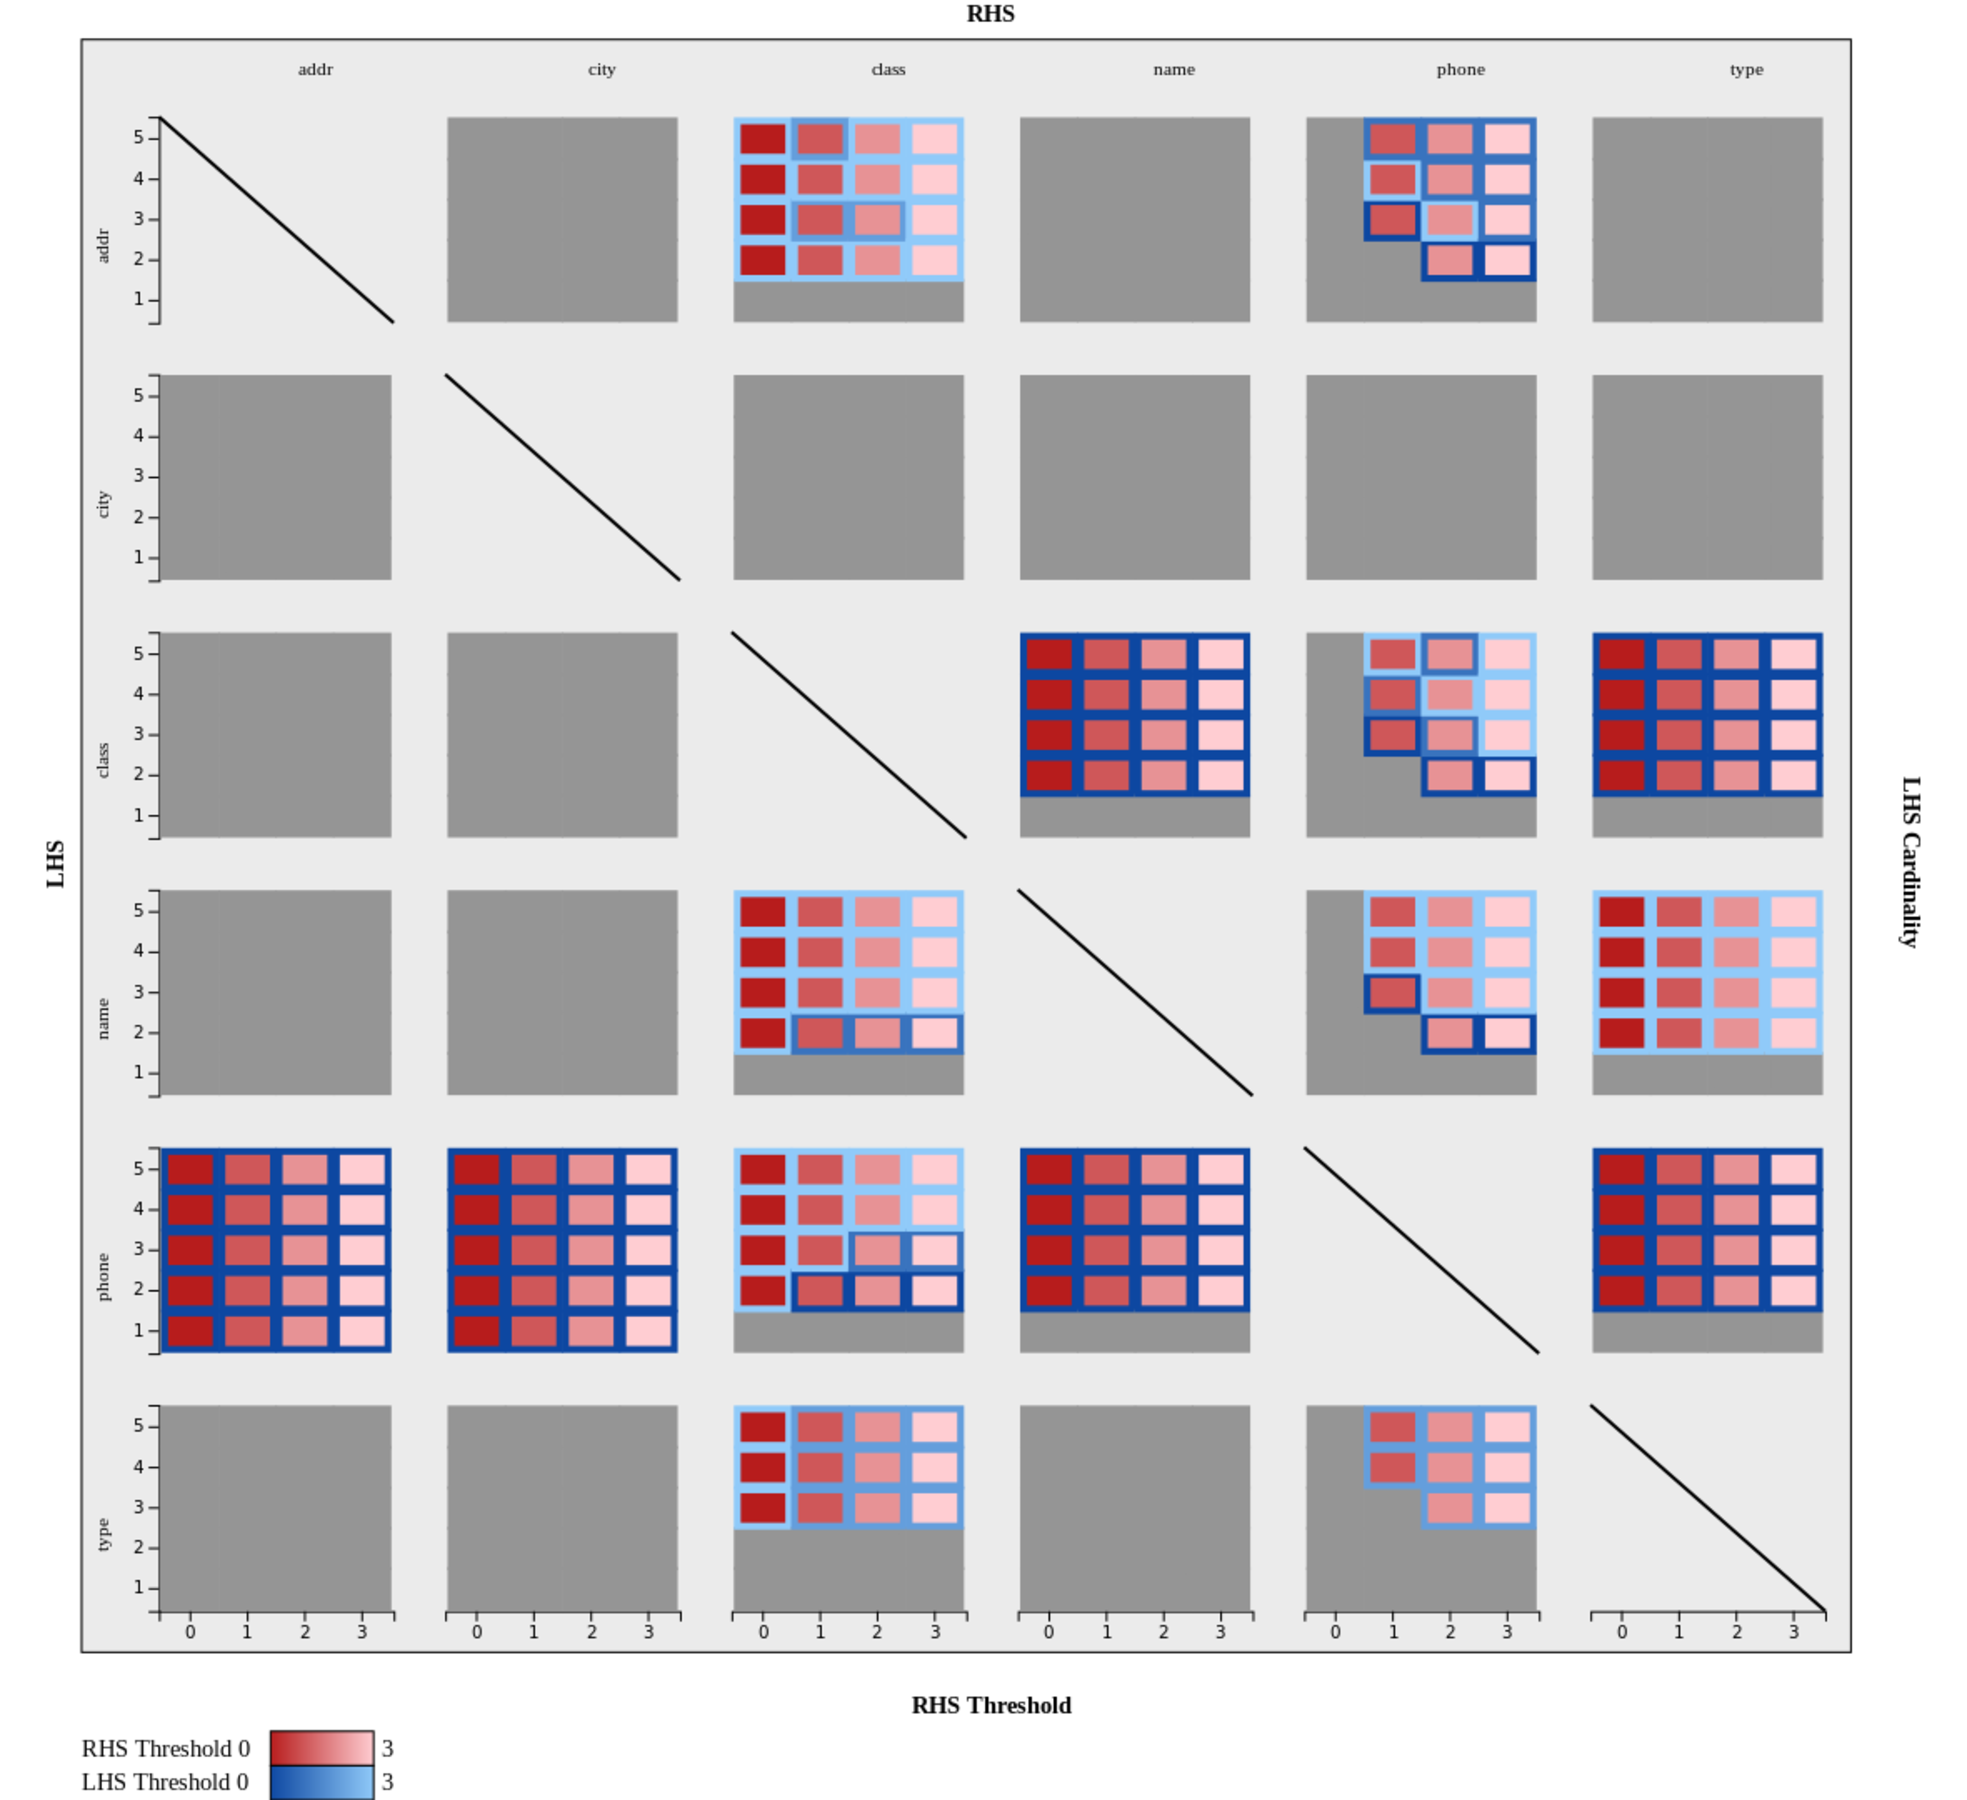
\includegraphics[width=\linewidth]{capitoli/figure/restaurant}
    \caption{Rappresentazione ottenuta in output da Dependensee del dataset Restaurant.}
    \label{fig:restaurant_result}
\end{figure}
Per quanto concerne l'analisi del dataset \textit{Restaurant}, la Figura \ref{fig:restaurant_result} mostra la rappresentazione grafica ottenuta mediante l'utilizzo di Dependensee. Da un'analisi generale si pu\`{o} affermare che le \acrlong{rfds} minimimali esistenti sono distribuite e non coprono tutti gli attributi del dataset. Infatti, la seconda riga \`{e} totalmente grigia, segno che non esiste alcuna \acrlong{rfds} minimale con l'attributo \texttt{city} sul lato sinistro. Continuando, vi sono molte altre sotto-matrici grigie che indicano l'assenza di \acrlong{rfds} minimali. Ci\`{o} non \`{e} uguale per tutte le sotto-matrici del grafico. Se consideriamo la riga relativa all'attributo \texttt{phone}, questa presenta \acrlong{rfds} minimali per tutti gli attributi. Le \acrlong{rfds} minimali con l'attributo \texttt{phone} sul lato sinistro, in relazione con gli attributi \texttt{addr}, \texttt{city}, \texttt{name} e \texttt{type} sul lato destro, sono tutte threshold minima sul lato sinistro. Mentre, la maggior parte di quelle in relazione con l'attributo \texttt{class} sul lato destro hanno threshold massima, alcune hanno threshold minima o quasi. Se, invece, consideriamo la terza colonna relativa all'attributo \texttt{class} sul lato destro, possiamo notare che quasi tutte le \acrlong{rfds} minimali hanno threshold massima o molto vicina a questa sul lato sinistro. Invece, la colonna relativa all'attributo \texttt{addr} sul lato destro, presenta solo \acrlong{rfds} minimali con threshold minima sul lato sinistro in relazione con l'attributo \texttt{phone}. Considerando, invece, la colonna relativa all'attributo \texttt{name} sul lato destro, presenta solo \acrlong{rfds} minimali con threshold minima sul lato sinistro relative agli attributi \texttt{class} e \texttt{phone}. Invece, l'ultima colonna relativa all'attributo \texttt{type} presenta \acrlong{rfds} minimali solo con gli attributi \texttt{class}, \texttt{name} e \texttt{phone}. Quelle relative agli attributi \texttt{class} e \texttt{phone} sul lato destro sono tutte con threshold minima, mentre quelle relative all'attributo \texttt{name} sono tutte con threshold massima.\par
\begin{figure}[ht]
    \centering
    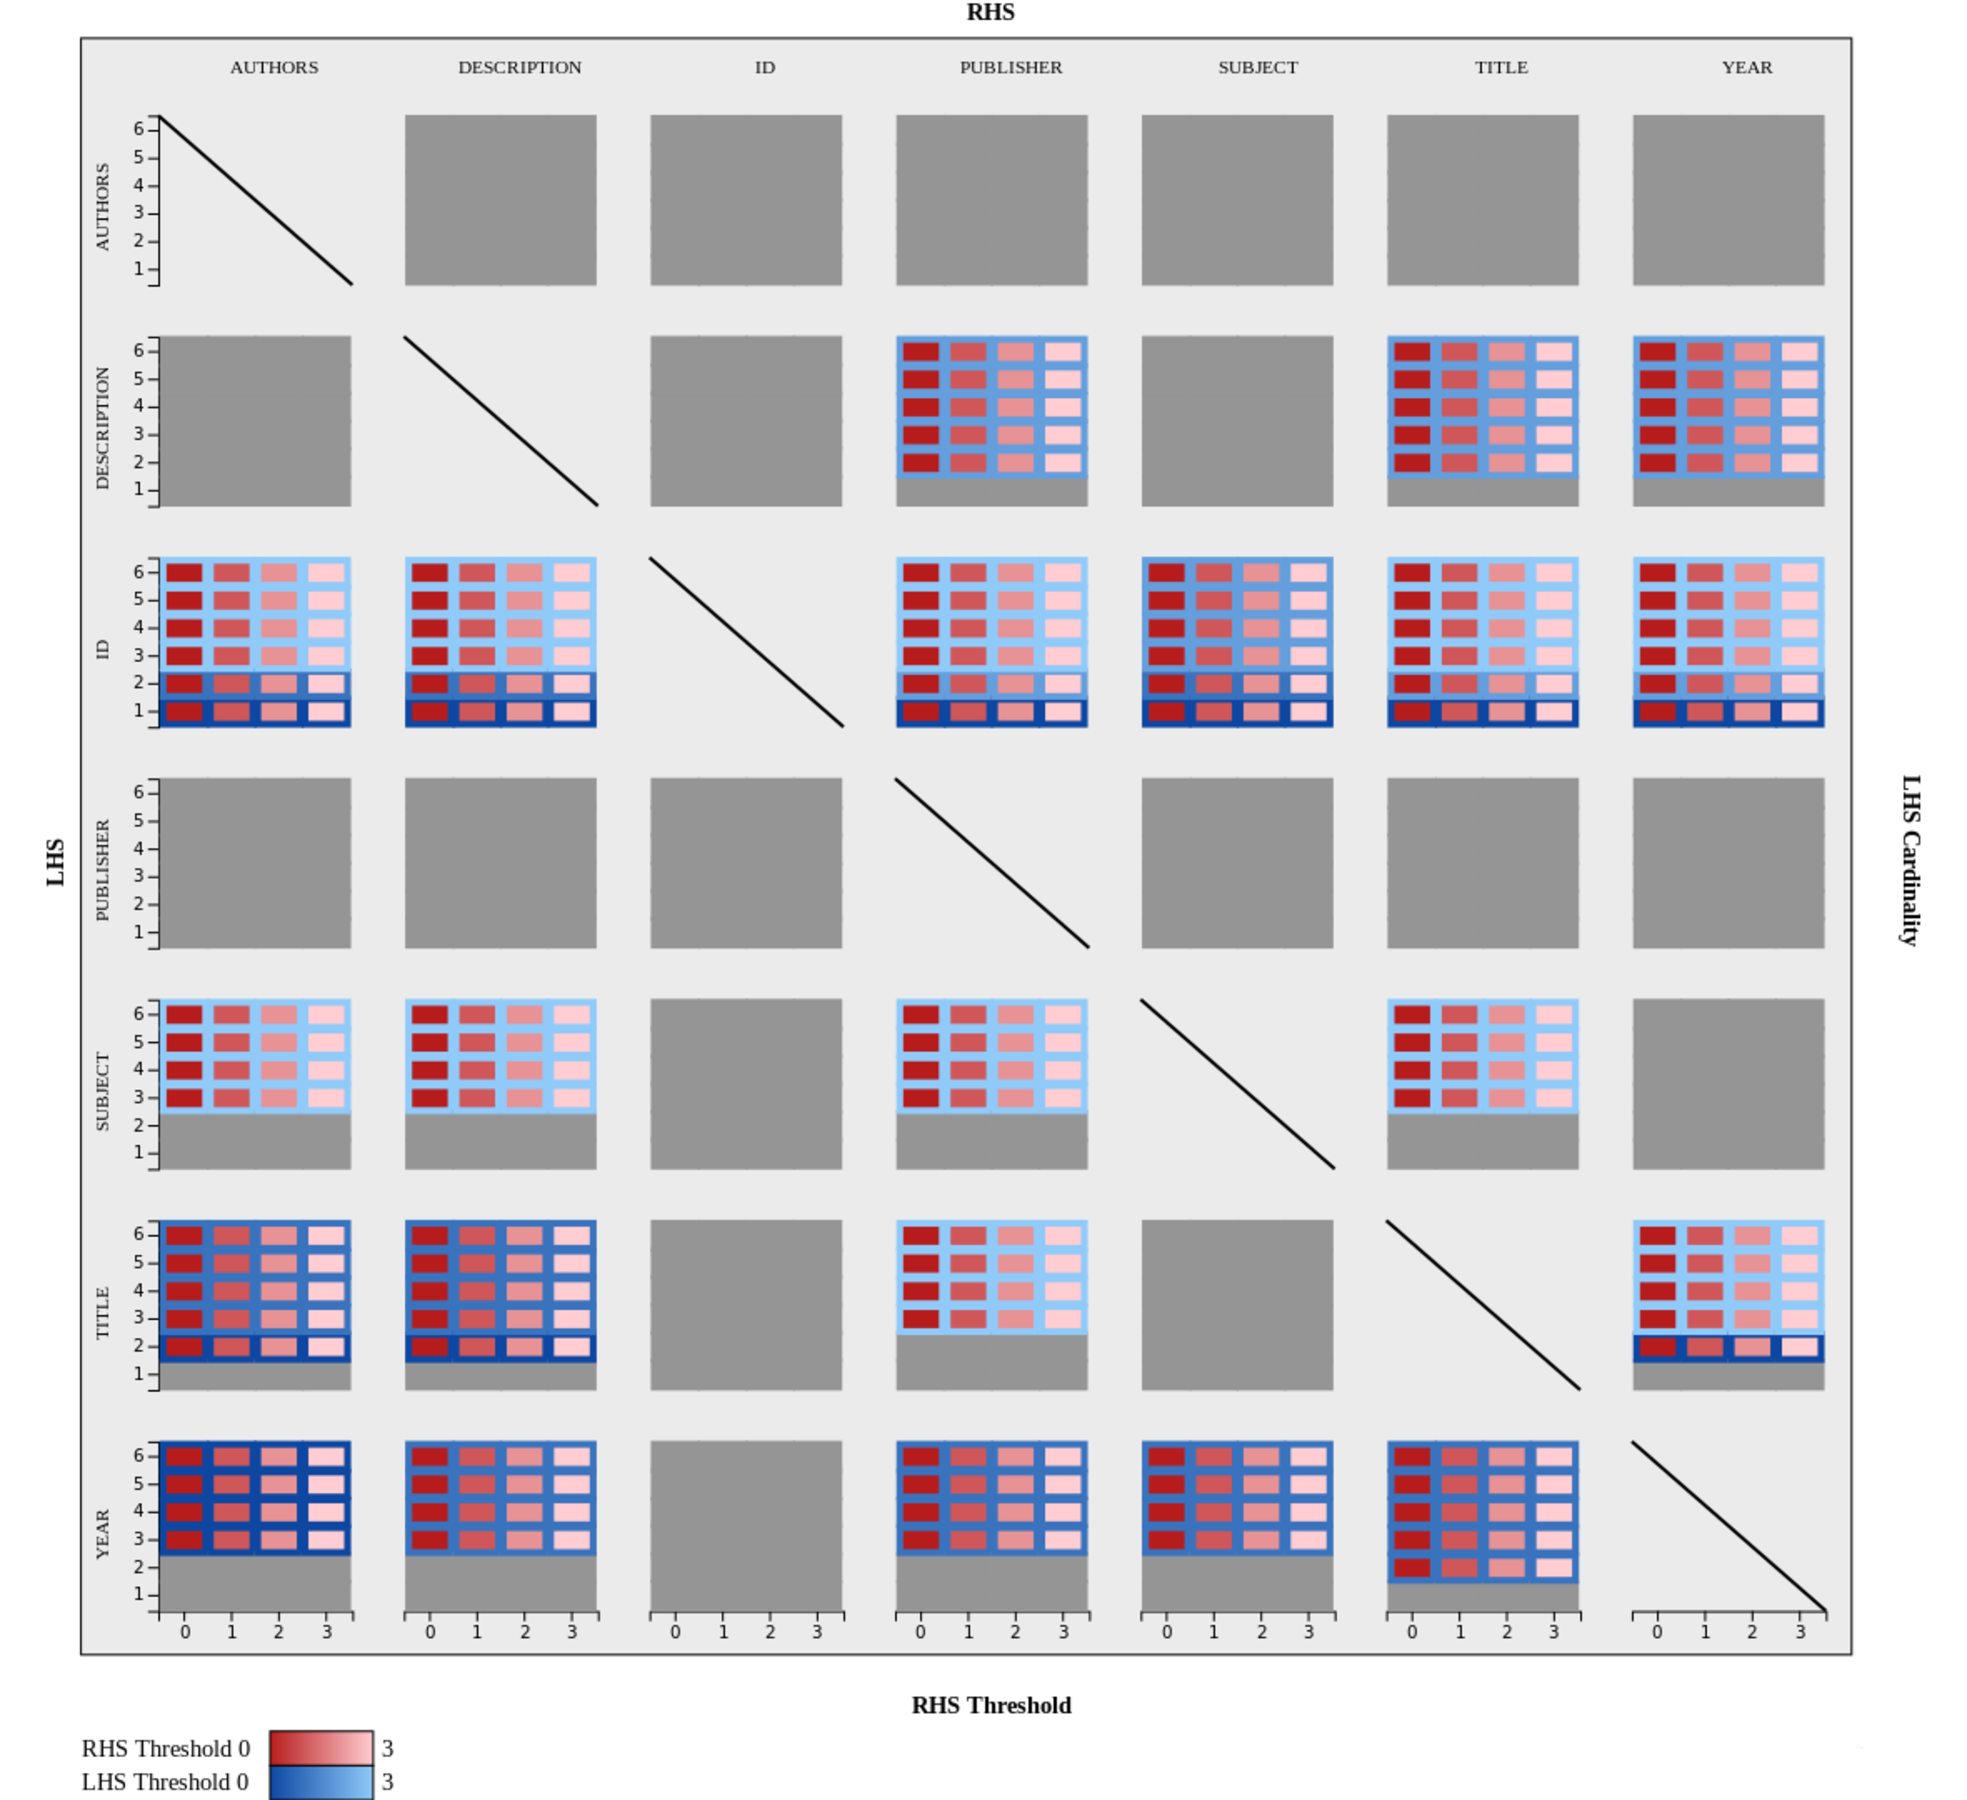
\includegraphics[width=\linewidth]{capitoli/figure/citiseer_2000_result}
    \caption{Rappresentazione ottenuta in output da Dependensee del dataset Citiseer 2000.}
    \label{fig:citiseer_2000_result}
\end{figure}
La Figura \ref{fig:citiseer_2000_result} mostra la rappresentazione grafica ottenuta analizzando il dataset \textit{Citiseer 2000} con Dependensee. Visto il basso numero di attributi, il grafico mostrer\`{a} anche il colore di riempimento relativo alla threshold del lato destro. Se prendiamo in considerazione la prima riga, possiamo notare come non esistano \acrlong{rfds} minimali con l'attributo \texttt{AUTHORS} sul lato sinistro e con almeno un attributo diverso sul lato destro, infatti tutta la riga \`{e} grigia. Analogamente con la terza riga, relativa all'attributo \texttt{PUBLISHER}. Mentre, con la colonna relativa all'attributo \texttt{ID}, possiamo notare l'assenza di \acrlong{rfds} minimali con l'attributo relativo sul lato destro. Se analizziamo la sotto-matrice relativa all'attributo riga \texttt{TITLE} ed all'attributo colonna \texttt{AUTHORS}, possiamo notare l'assenza di \acrlong{rfds} con cardinalit\`{a} pari a $1$ e l'esistenza di \acrlong{rfds} minimali con threshold pari a $0$ sul lato sinistro e cardinalit\`{a} pari a $2$, mentre per cardinalit\`{a} maggiori vi sono \acrlong{rfds} con threshold diverse da $0$ ma con valori vicini a questo. Pi\`{u} in generale, la prima riga mostra l'esistenza di \acrlong{rfds} minimali con valore di threshold vicino al massimo inserito per l'analisi, ovvero $3$. La terza riga, invece, mostra la vasta presenza di \acrlong{rfds} minimali, molte con threshold pari al minimo o vicino a questo. La quinta riga, invece, mostra l'esistenza di \acrlong{rfds} minimali, tutte con valore di threshold minimo. L'ultima riga, invece, rappresenta le \acrshort{rfds} minimali, tutte con valore della threshold uguale al minino o vicino a questo.\par
\begin{figure}[ht]
    \centering
    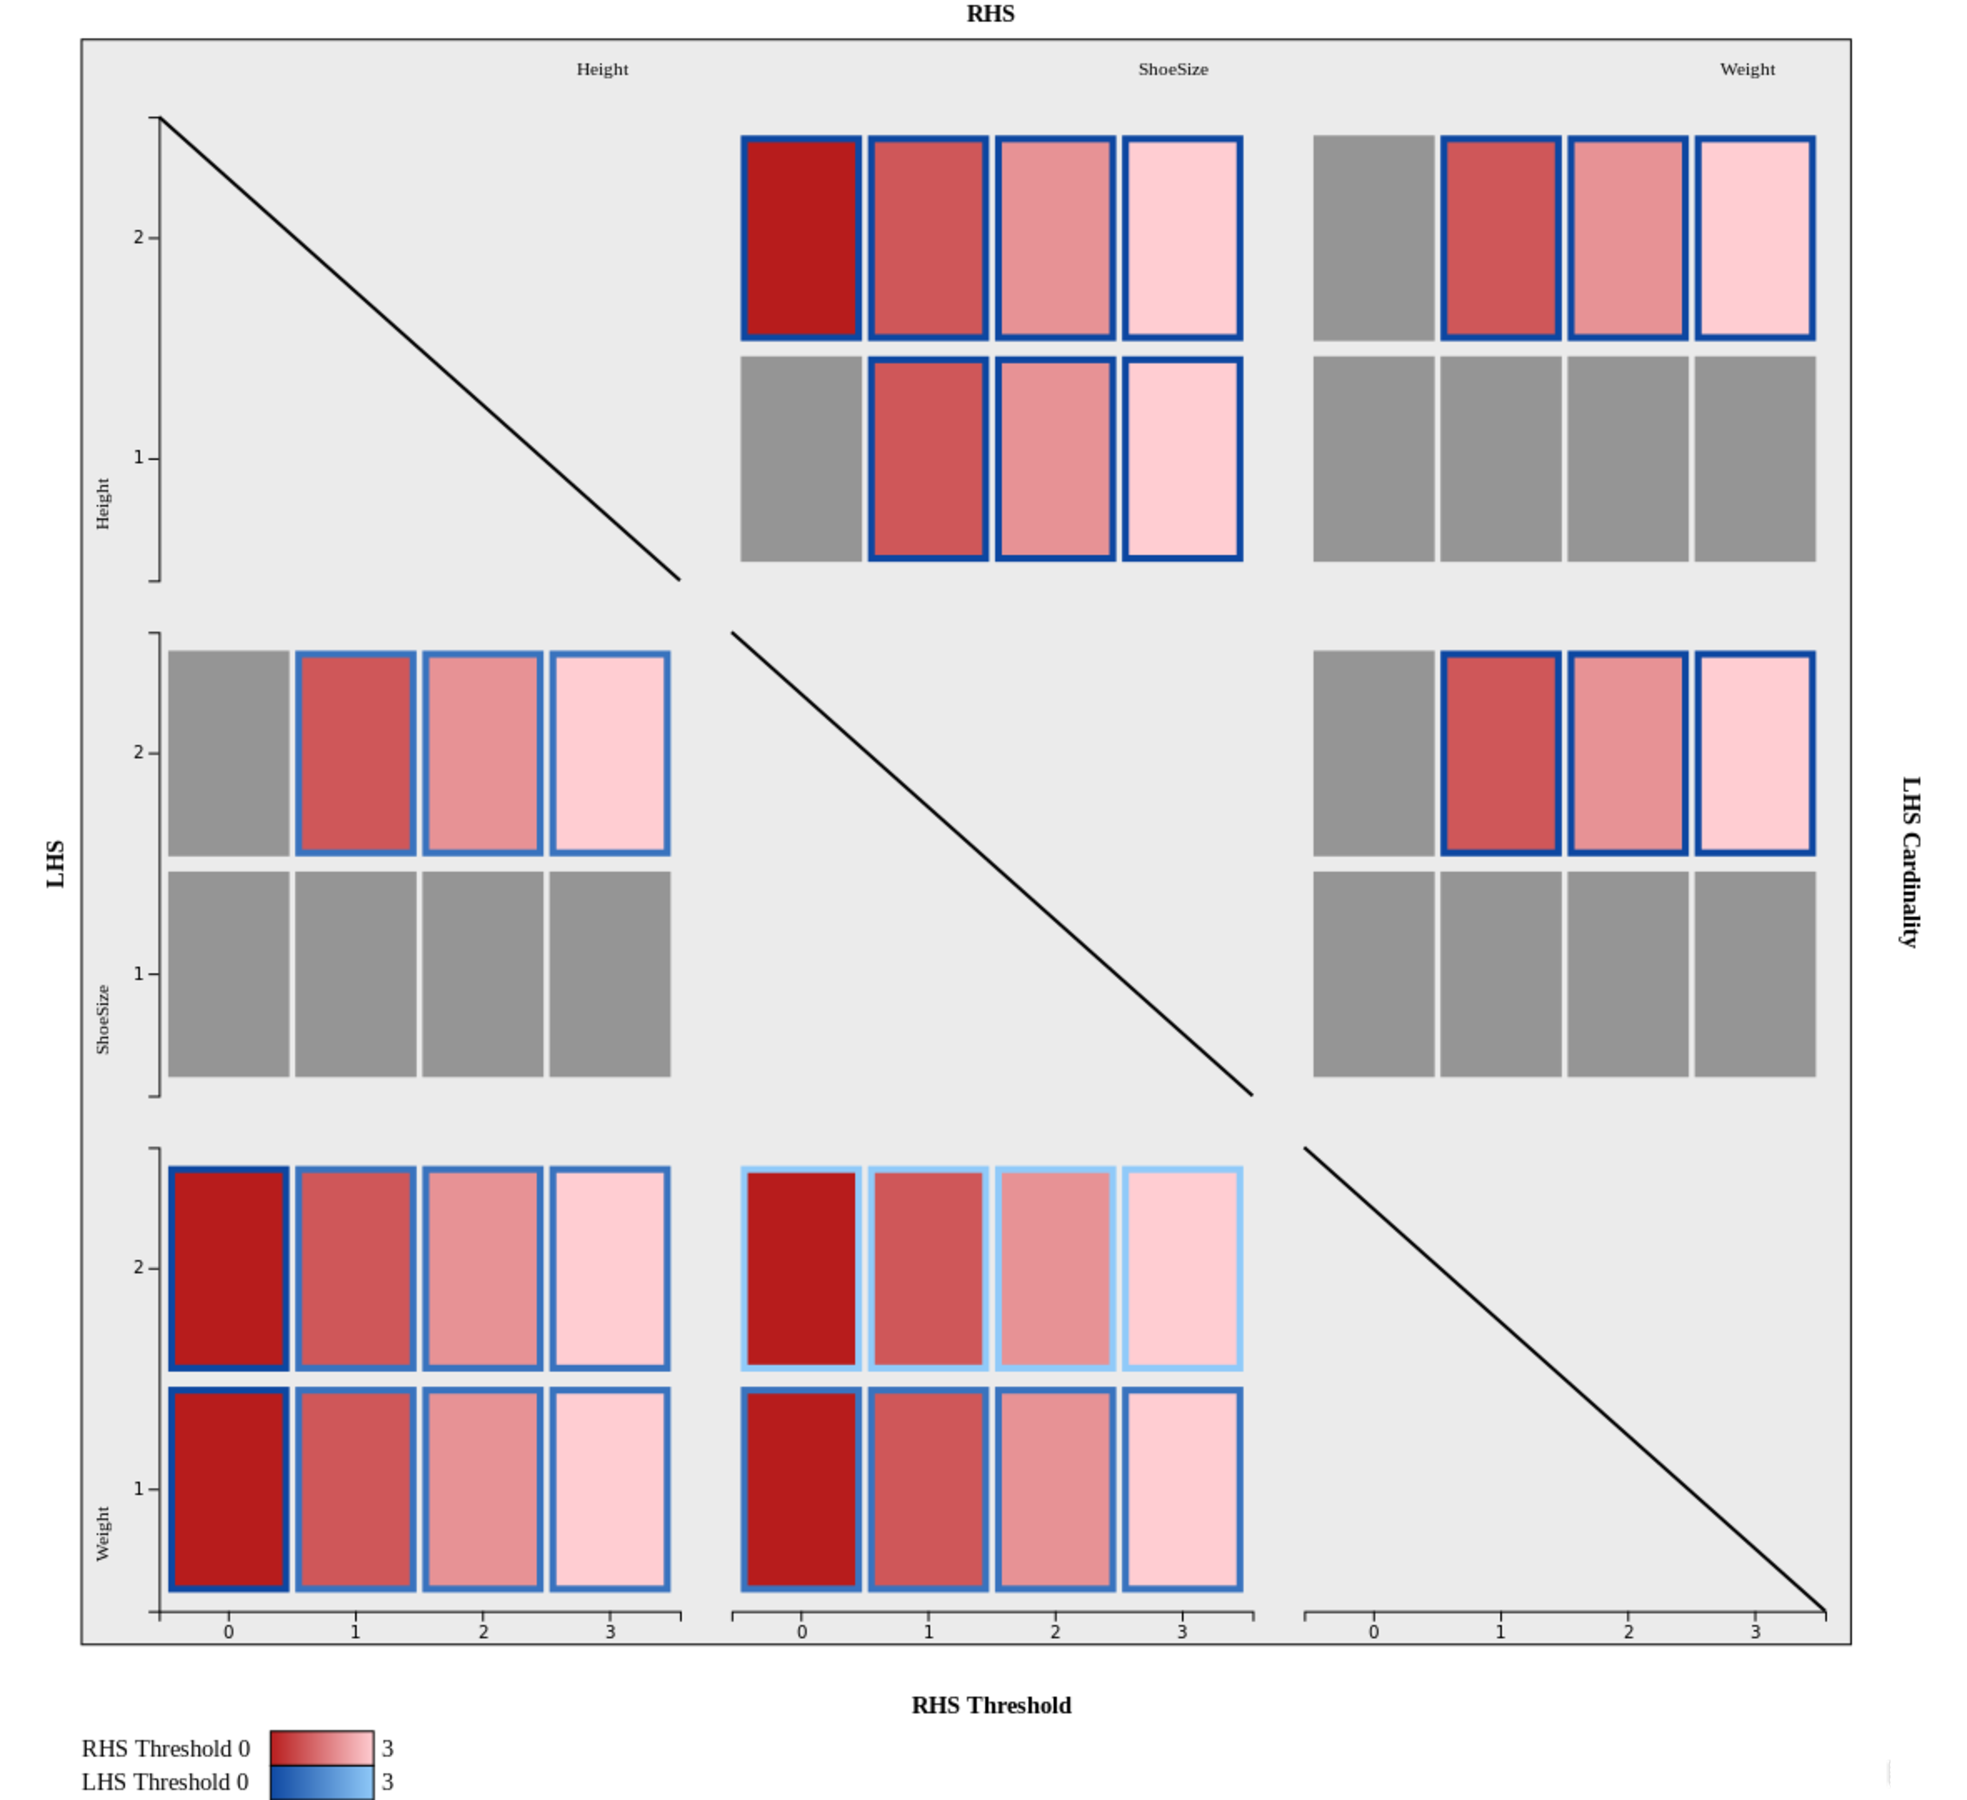
\includegraphics[width=\linewidth]{capitoli/figure/expIDEAS}
    \caption{Rappresentazione ottenuta in output da Dependensee del dataset expIDEAS.}
    \label{fig:expidea_result}
\end{figure}
La Figura \ref{fig:expidea_result} rappresenta il grafico ottenuto analizzando il dataset \textit{expIDEAS} mediante Dependensee. Il dataset contiene soltanto $3$ attributi e $12$ \acrlong{rfds} minimali. Dalla rappresentazione si pu\`{o} notare che le \acrlong{rfds} minimali sono ben distribuite. Con la prima riga possiamo notare che l'attributo \texttt{Height} sul lato sinistro figura in \acrlong{rfds} minimali con threshold minima. Anche con l'ultima colonna possiamo notare che l'attributo \texttt{Weight} sul lato destro figura in \acrlong{rfds} minimali con threshold minima. Invece, con l'ultima riga si pu\`{o} notare che l'attributo \texttt{Weight} sul lato sinistro figura in \acrlong{rfds} minimali, molte delle quali con threshold vicino o pari al massimo e poche con threshold pari al minimo.\par
\begin{figure}[ht]
    \centering
    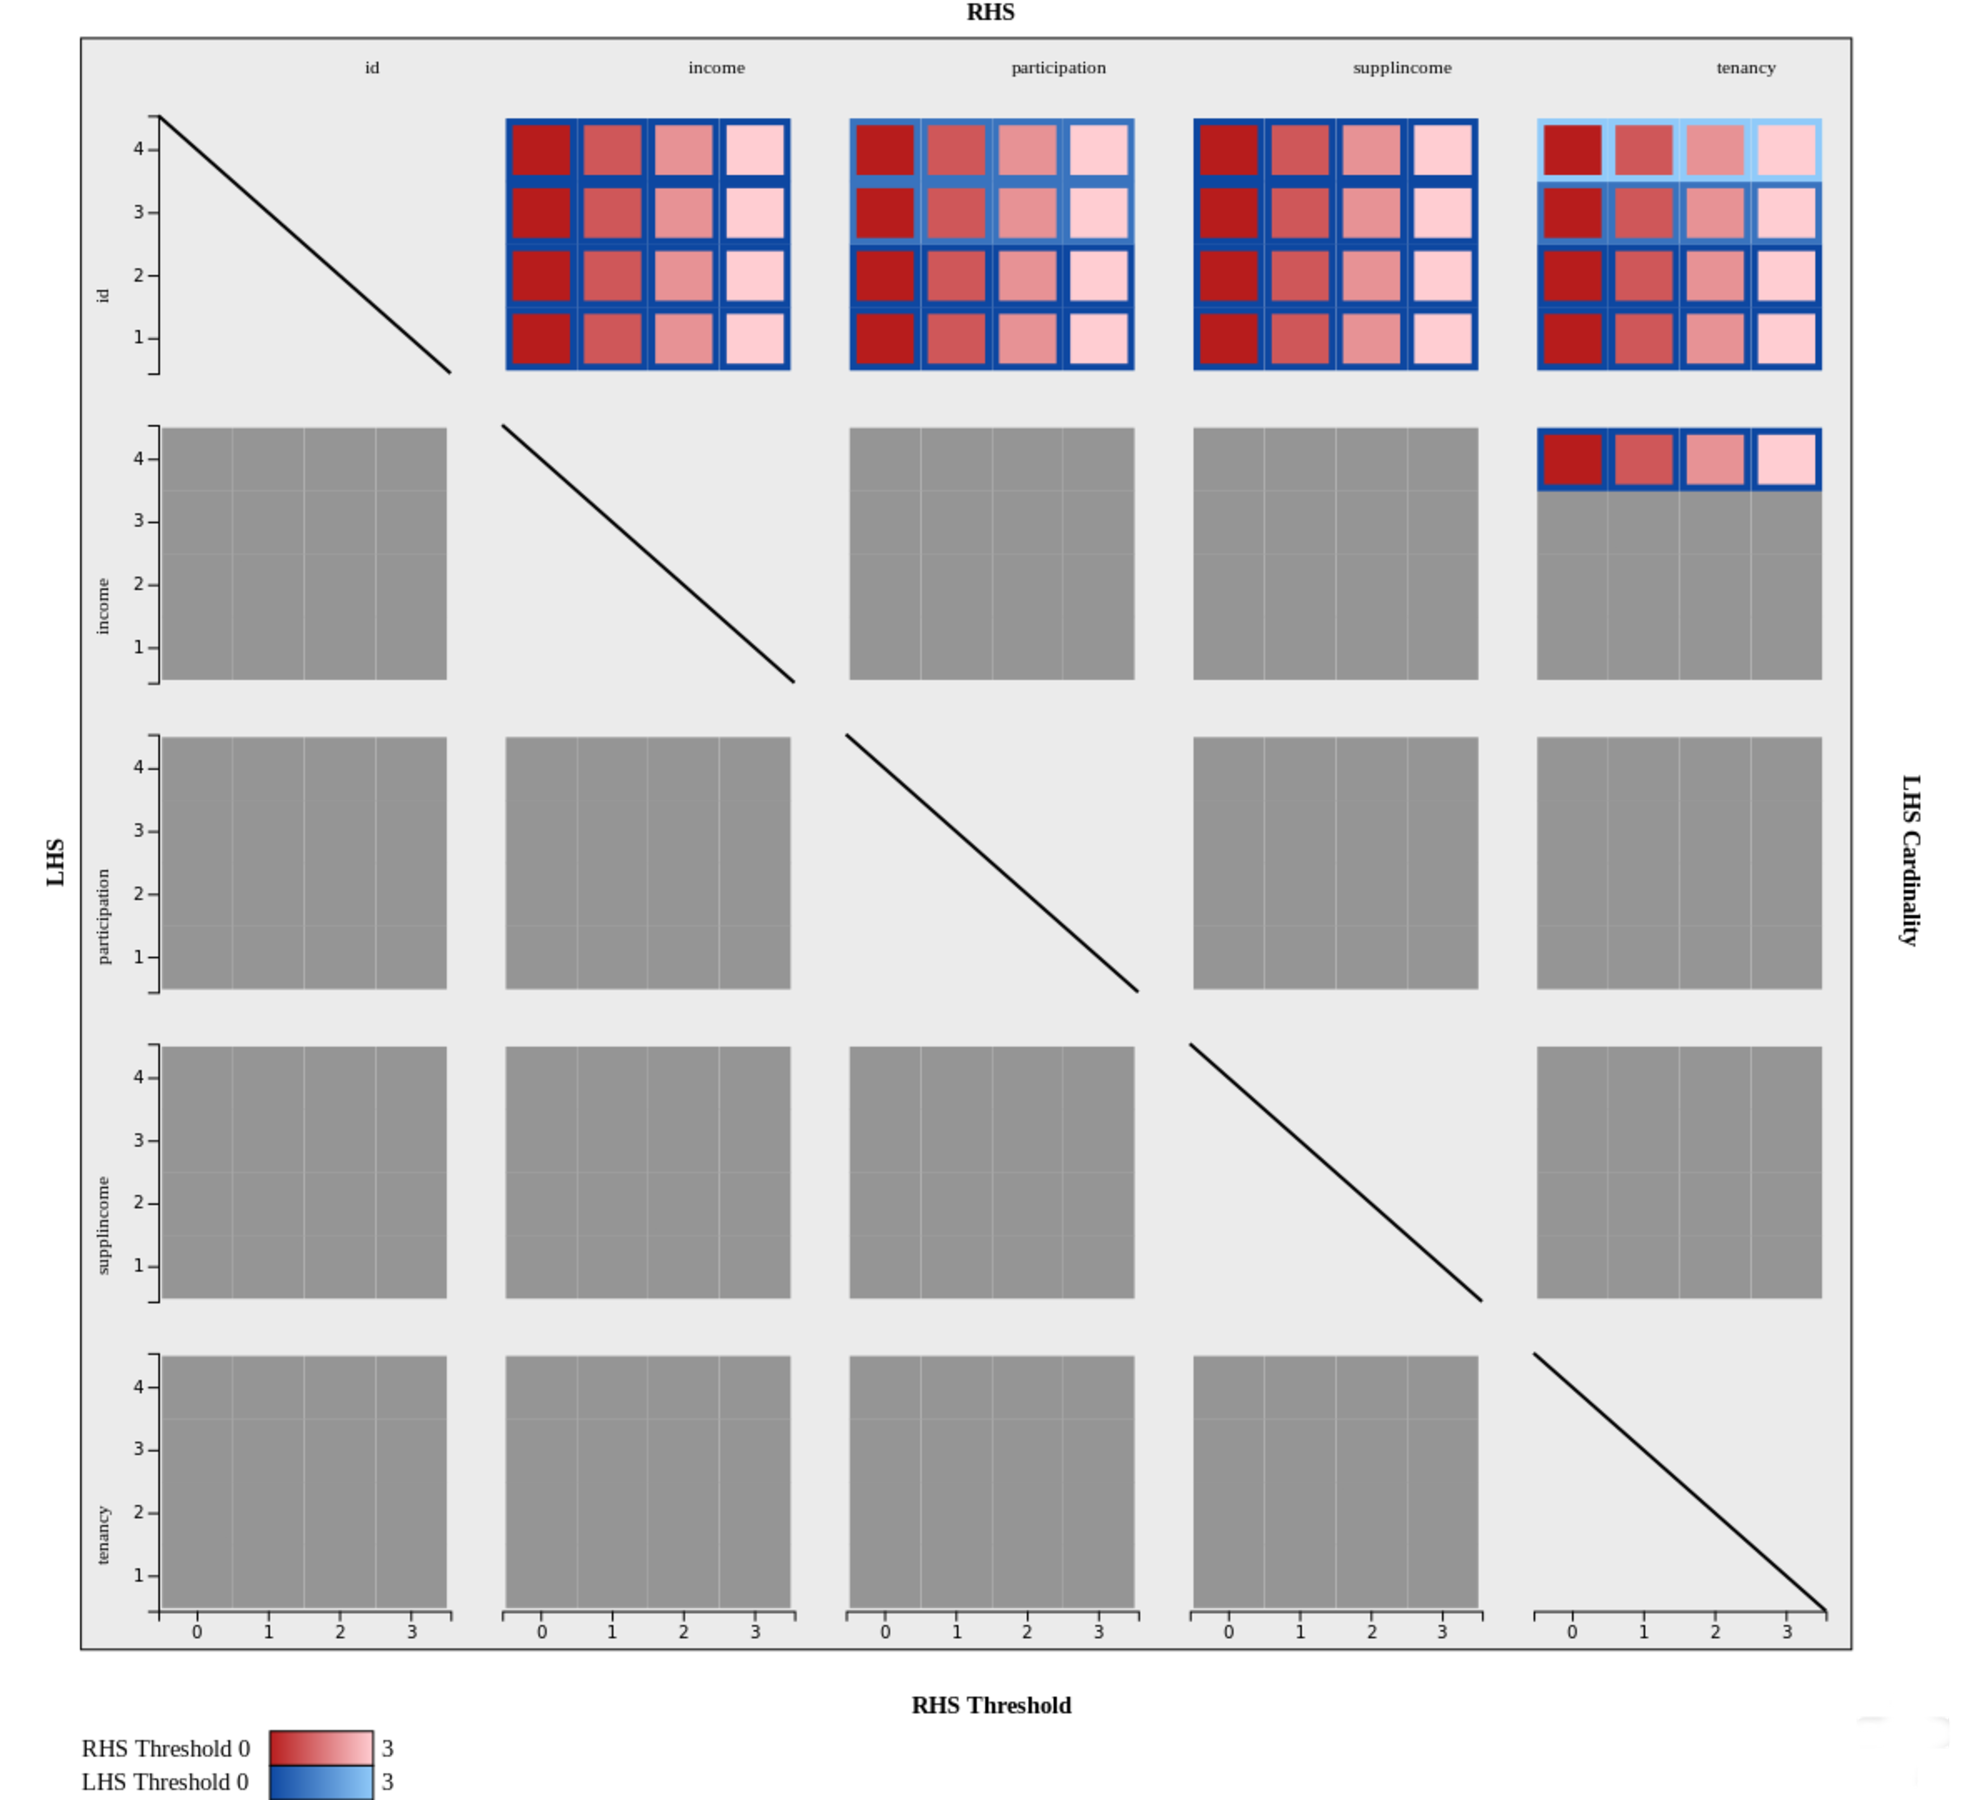
\includegraphics[width=\linewidth]{capitoli/figure/foodstamp_result}
    \caption{Rappresentazione ottenuta in output da Dependensee del dataset Foodstamp.}
    \label{fig:foodstamp_result}
\end{figure}
Consideriamo adesso il dataset \textit{Foodstamp}. La Figura \ref{fig:foodstamp_result} mostra la rappresentazione grafica ottenuta dando in input il dataset a Dependensee. Dal grafico ottenuto possiamo notare, attraverso la prima riga, come le uniche dipendenze esistenti siano con l'attributo \texttt{id} sul lato sinistro e, attraverso la seconda riga, con l'attributo \texttt{income} sul lato sinistro. Le prime sono in relazione con tutti gli altri attributi del dataset, infatti le colonne relative alla prima riga sono tutte colorate. Mentre, per l'attributo \texttt{income}, possiamo notare l'esistenza di \acrlong{rfds} solo con l'attributo \texttt{tenancy} sul lato destro. Le \acrlong{rfds} minimali presenti hanno quasi tutte una threshold minima o quasi, tranne quelle relative all'attributo \texttt{id} sul lato sinistro e l'attributo \texttt{tenancy} sul lato destro, le quali hanno threshold e cardinalit\`{a} massima. Con le righe e le colonne restanti possiamo notare che non vi sono \acrlong{rfds}, difatti sono colorate in grigio.\par
\begin{figure}[ht]
    \centering
    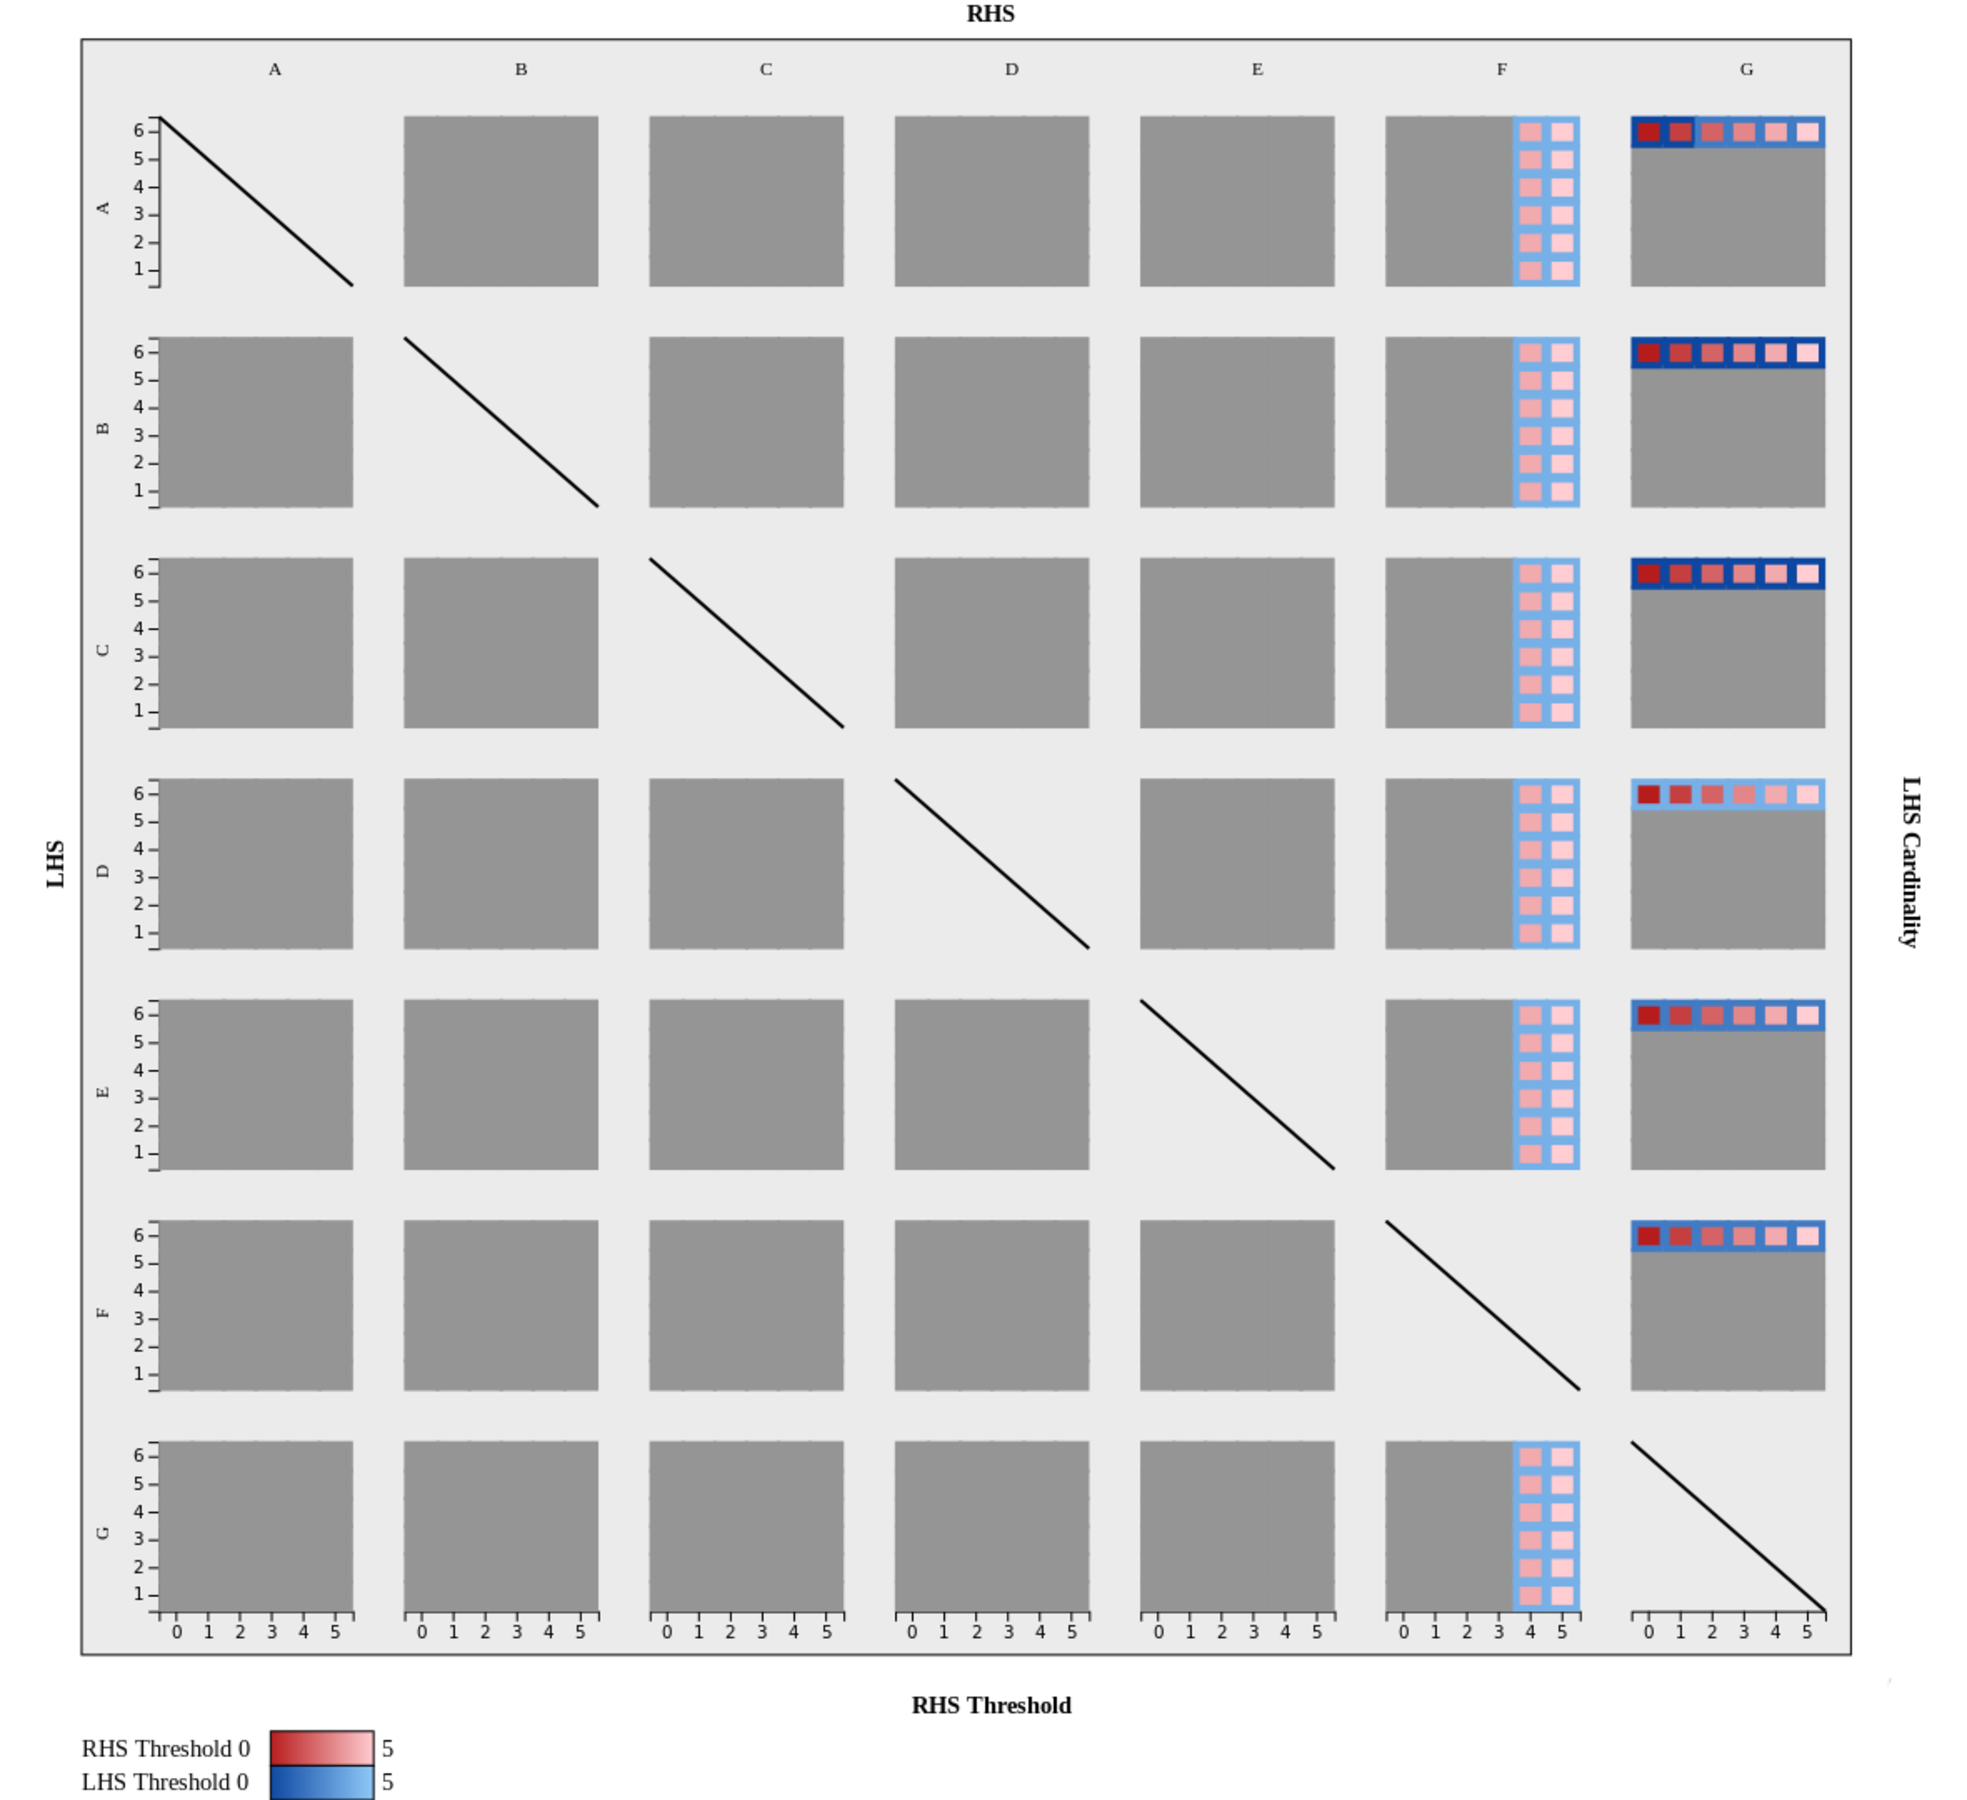
\includegraphics[width=\linewidth]{capitoli/figure/car_data}
    \caption{Rappresentazione ottenuta in output da Dependensee del dataset Car Data.}
    \label{fig:cardata_result}
\end{figure}
Il dataset \textit{Car\_Data} \`{e} stato analizzato con una threshold massima data in input pari a $5$. Le \acrlong{rfds} minimali presenti in questo dataset son poche e la maggior parte hanno una threshold alta. Se prendiamo in considerazione la colonna relativa all'attributo \texttt{F}, possiamo notare che le \acrlong{rfds} minimali esistenti siano tutte con una threshold sul lato sinistro pari a $5$ e threshold sul lato destro pari a $4$ e $5$. Se consideriamo, invece, la colonna relativa all'attributo \texttt{G}, possiamo notare che le \acrlong{rfds} minimali esistenti sono tutte con cardinalit\`{a} massima, con threshold massima o quasi sul lato sinistro e con threshold tra $0$ e $5$ sul lato destro.